\documentclass[a4paper, 12pt, twoside, openright, fleqn]{book}

% language settings
\usepackage[english]{babel}
\usepackage[T1]{fontenc}

\usepackage[utf8]{inputenc}
\usepackage{textgreek}

\usepackage{fancyhdr} % headers and footers

% figures and positioning
\usepackage{caption}
\usepackage{float}
\usepackage{graphicx}
\usepackage{graphics}
\usepackage{wrapfig}
\usepackage{listing}
%\usepackage{rotating}

% math package
\usepackage{mathtools}
\usepackage{amsthm, environ}
\usepackage{amsmath, amssymb, dsfont, bm,blkarray}
\usepackage{cases}

% tikz figures
\usepackage[usenames, dvipsnames, table, tikz]{xcolor}
\usepackage{tikz}
\usetikzlibrary{shapes, arrows,automata}

% image path
\graphicspath{ {./img/} }

% add support for url and cross-references in PDF output
\usepackage{url}
\renewcommand{\UrlFont}{\color{black}\small\ttfamily}
\usepackage[colorlinks=true, linkcolor=black, citecolor=black, urlcolor=black]{hyperref}

% support for glossary and acronyms
\usepackage[acronym]{glossaries}
\newacronym[plural=MCs,firstplural=Markov Chains (MCs)]{mc}{MC}{Markov Chain}

% Costumization of theorem style
\newtheoremstyle{theoremdd}% name of the style to be used
  {\topsep}% measure of space to leave above the theorem. E.g.: 3pt
  {\topsep}% measure of space to leave below the theorem. E.g.: 3pt
  {\itshape}% name of font to use in the body of the theorem
  {0pt}% measure of space to indent
  {\bfseries}% name of head font %\color{Mahogany}
  { -- }% punctuation between head and body
  { }% space after theorem head; " " = normal interword space
  {\thmname{#1}\thmnumber{ #2}\thmnote{ (#3)}}

\theoremstyle{theoremdd}
% support for counting
\newtheorem{theorem}{Theorem}[section]
\newtheorem{corollary}{Corollary}[theorem]
\newtheorem{lemma}[theorem]{Lemma}
\newtheorem{definition}{Definition}
\newtheorem{remark}{Remark}

% added support for proof parts
\theoremstyle{remark}
\newtheorem{proofpart}{Part}
\renewcommand\theproofpart{\Roman{proofpart}}
\makeatletter
\@addtoreset{proofpart}{theorem}
\makeatother

% specific modification to basic book template of our book document
\renewcommand{\chaptername}{Section}
\addto\captionsenglish{\renewcommand{\chaptername}{Section}}
\renewcommand\qedsymbol{
\includegraphics[width=1.5cm]{occhiali}}
%\renewcommand\qedsymbol{$\square$\itshape QED}


% useful aliases for common employed declarations
\def \beq {\begin{equation}}
\def\eeq{\end{equation}}
\def\bal{\begin{align}}
\def\eal{\end{align}}
\def\prob{\ensuremath\mathbb{P}}
\def\exp{\ensuremath\mathbb{E}}
\newcommand{\Hb}{\mathbb{H}}
\newcommand{\Sb}{\mathbb{\Sigma}}
\newcommand{\U}{\mathbb{U}}
\newcommand{\F}{\mathbb{F}}
\newcommand{\V}{\mathbb{V}}
\newcommand{\A}{\mathbb{A}}
\newcommand{\B}{\mathbb{B}}
\newcommand{\C}{\mathbb{C}}
\newcommand{\E}{\mathbb{E}}
\newcommand{\I}{\mathbb{I}}
\newcommand{\Y}{\mathbb{Y}}
\newcommand{\N}{\mathbb{N}}
\newcommand{\W}{\mathbb{W}}
\newcommand{\Z}{\mathbb{Z}}
\newcommand{\R}{\mathbb{R}}
\newcommand{\X}{\mathbb{X}}
\newcommand{\Pb}{\mathbb{P}}
\newcommand{\Q}{\mathbb{Q}}
\newcommand{\D}{\mathbb{D}}
\newcommand{\Rm}{\mathbb{R^{-1}}}
\newcommand{\J}{\mathbb{J}}
\newcommand*{\Chi}{\mbox{\Large $\chi$}}% big chi
\newcommand{\Fig}[1]{Fig.~\ref{#1}}
\newcommand{\eq}[1]{(\ref{#1})}
\newcommand{\Tab}[1]{Tab.~\ref{#1}}
\newcommand{\Sec}[1]{Sec.~\ref{#1}}
\newcommand{\indep}{\mathrel{\perp\mspace{-10mu}\perp}}
\newcommand{\RN}[1]{ \textup{\uppercase\expandafter{\romannumeral#1}}} %This is for inserting Roman Numbers (useful for \stackrel in equations so that you don't confuse indicating numbers from equation numbers
\newcommand{\e}{\ensuremath{\vec{e}}}
\newcommand{\ert}{\ensuremath{\vec{e}(\vec{r},t)}}
\renewcommand{\b}{\ensuremath{\vec{b}}}
\newcommand{\brt}{\vec{b}(\vec{r},t)}
\newcommand{\h}{\ensuremath{\vec{h}}}
\newcommand{\hrt}{\ensuremath{\vec{h}(\vec{r},t)}}
\renewcommand{\d}{\ensuremath{\vec{d}}}
\newcommand{\drt}{\ensuremath{\vec{d}(\vec{r},t)}}
\newcommand{\jt}{\ensuremath{\vec{j}_T}}
\renewcommand{\r}{\ensuremath{\vec{r}}}
\newcommand{\s}{\ensuremath{\vec{s}}}
\renewcommand{\a}{\ensuremath{\vec{a}}}
\renewcommand{\k}{\ensuremath{\vec{k}}}
\newcommand{\rot}{\ensuremath{\nabla\times}}
\newcommand{\diverg}{\ensuremath{\nabla\cdot}}
\renewcommand{\E}{\ensuremath{\vec{E}}}
\renewcommand{\H}{\ensuremath{\vec{H}}}
\renewcommand{\J}{\ensuremath{\vec{J}}}

%Derivatives shortcut
\newcommand{\deriv}[3][]{% \deriv[<order>]{<func>}{<var>}
  \ensuremath{\frac{\partial^{#1} {#2}}{\partial {#3}^{#1}}}}
%---------------------------------
\NewEnviron{esp}{%
\begin{equation}\begin{split}
  \BODY
\end{split}\end{equation}
}

\begin{document}

\begin{titlepage}
	\begin{center}
		\hspace{0.5cm}
		\Large{Antenne e propagazione wireless} \\
		\vspace{1cm}
		%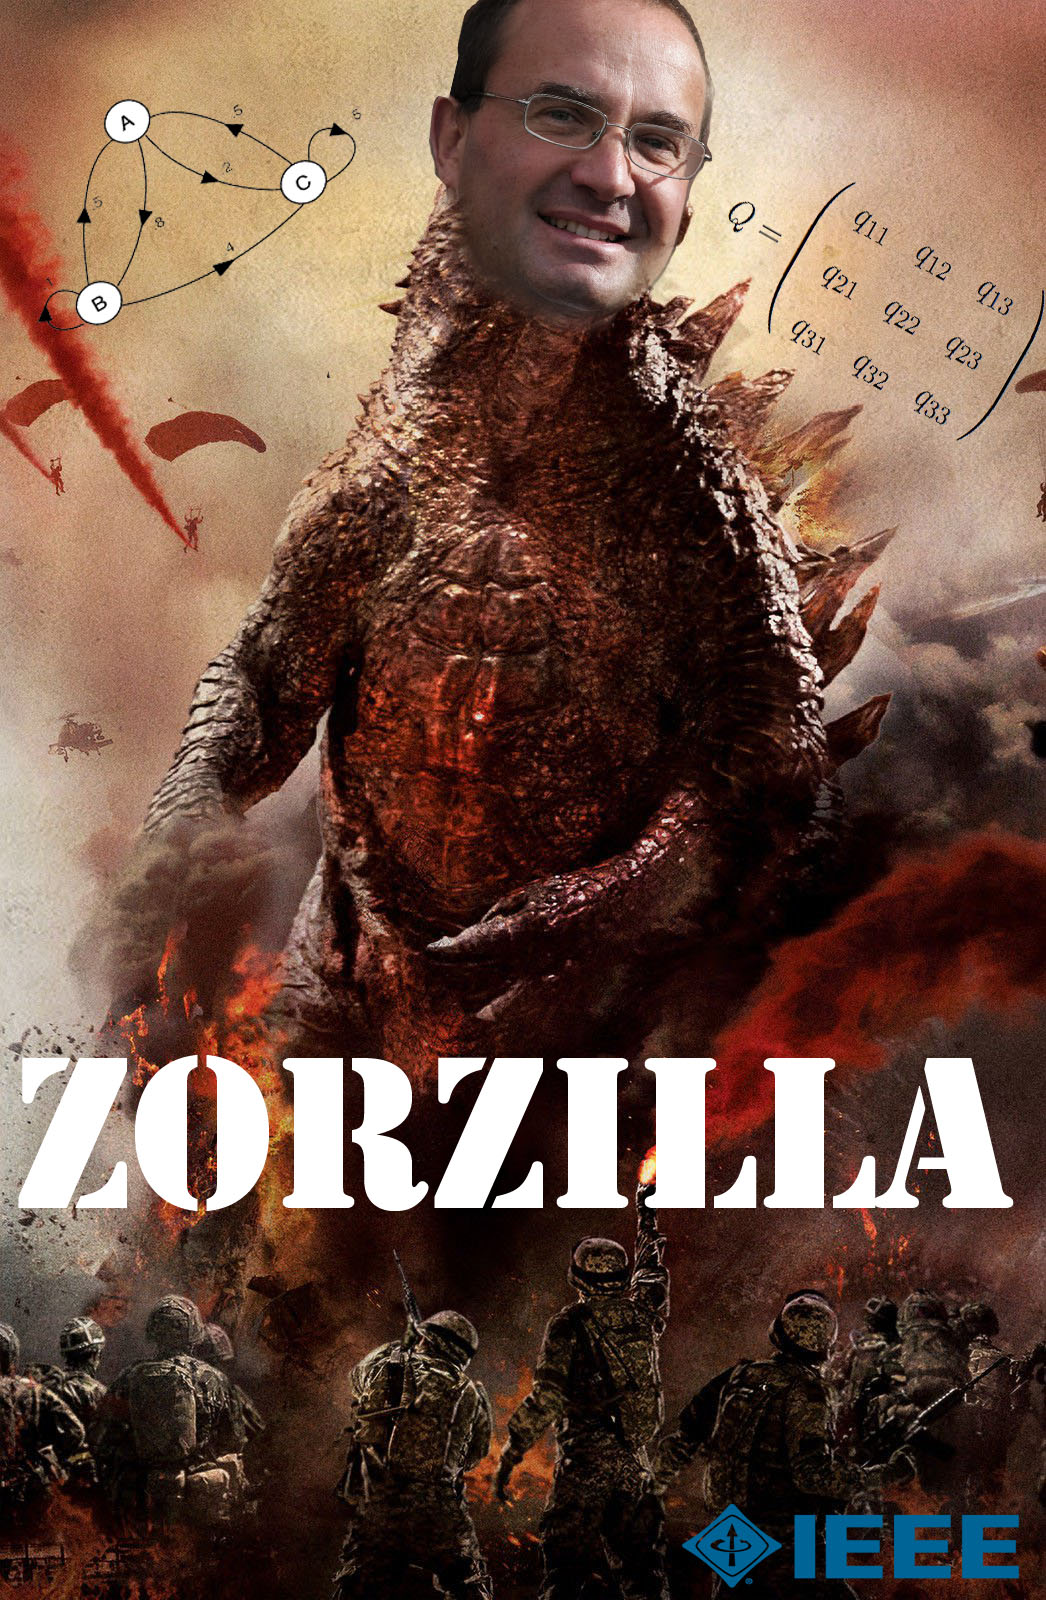
\includegraphics[width=9cm]{Zorzilla}\\
		\vspace{0.5cm}
		\emph{written with love by} \\
		\vspace{0.5cm}
		{\Large Andrea Pittaro, Enrico Lovisotto, Umberto Martinelli}
	\end{center}

	\vfill

	\begin{center}
		\line(1, 0){360}

		\textsc{Academic Year 2016/2017}
	\end{center}
\end{titlepage}

\tableofcontents
\clearpage

\chapter{Introduzione}
\section{Sistemi di riferimento}
Nel corso verranno utilizzate principalmente due sistemi di riferimento: quello
con coordinate \textbf{cartesiane} e quello con coordinate \textbf{sferiche}.
Le rappresentazioni di un punto \textit{\textbf{P}} nelle due coordinate saranno le seguenti:
\begin{equation}
  P=(x,y,z) = \r = x \cdot \hat{x} + y \cdot \hat{y} +z \cdot \hat{z}  \quad \r\text{ è il vettore posizione} \\
  x \bot y \bot z \bot x \\
  P=(r,\theta,\phi) = r \cdot \hat{r} = r \cdot \hat{r}(\theta,\phi)\\
  r \bot \theta \bot \phi \bot r
  \label{eq:riferimento}
\end{equation}

\section{Operatori differenziali (spaziali)}
Elenchiamo ora gli operatori che utilizzeremo, per poi definirli meglio in delle loro sottosezioni.
\begin{description}
  \item[Operatore Nabla] $ \nabla = \left(\frac{\partial}{\partial x},\frac{\partial}{\partial y},\frac{\partial}{\partial z}\right)$
  \item[Rotore] $\rot$
  \item[Divergenza] $\diverg$
  \item[Gradiente] $\nabla$
  \item[Laplaciano] $\nabla^2$
\end{description}
Iniziamo a descrivere cosa succede a un generico vettore $\vec{A}\left(\r\right)=\left(A_x(\r),A_y(\r),A_z(\r)\right)$.
\subsection{Rotore}
\begin{equation} \begin{split}
  \rot \vec{A(\r)} &=
  \begin{vmatrix}
    \hat{x} &\hat{y} &\hat{z} \\
    \frac{\partial}{\partial x} & \frac{\partial}{\partial y} & \frac{\partial}{\partial z} \\
    A_x & A_y & A_z
  \end{vmatrix} \\
  &= \left(\frac{\partial A_z}{\partial y} - \frac{\partial A_y}{\partial z}\right)\cdot \hat{x} -
  \left(\frac{\partial A_z}{\partial x} - \frac{\partial A_x}{\partial z}\right)\cdot \hat{y} +
  \left(\frac{\partial A_y}{\partial x} - \frac{\partial A_x}{\partial y}\right)\cdot \hat{z}
\end{split}\end{equation}

\subsection{Divergenza}
\begin{equation}
  \diverg \vec{A} = \frac{\partial A_x}{\partial x} + \frac{\partial A_y}{\partial y} + \frac{\partial A_z}{\partial z}
\end{equation}
\subsection{Gradiente}
Dato $\Phi(\r)$ uno scalare, il suo gradiente risulta
\begin{equation}
  \nabla \Phi = \left(\frac{\partial \Phi}{\partial x} ; \frac{\partial \Phi}{\partial y}; \frac{\partial \Phi}{\partial z}\right)
\end{equation}
\subsection{Laplaciano}
Dato $\Phi(\r)$ uno scalare, il suo laplaciano risulta
\begin{equation}
  \nabla^2 \Phi = \left(\frac{\partial^2 \Phi}{\partial x^2} + \frac{\partial^2 \Phi}{\partial y^2} + \frac{\partial^2 \Phi}{\partial z^2}\right)
\end{equation}

\section{Teoremi importanti}
Mostreremo ora due teoremi che verranno utilizzati per risolvere le equazioni di Maxwell:
il teorema di \textbf{Stokes} (o \textit{del rotore}) e il teorema di \textbf{Gauss} (del flusso).
Si mostrerà solo il risultato, senza enunciarlo nè dimostrarlo.
\subsection{Teorema di Stokes}
Data $\vec{l}$ una circuitazione, $S_l$ la superficie della circuitazione, $\hat{n}$
 il versore normale alla superficie  e $\vec{A}$ il vettore del campo attraverso la superficie $S_l$, si ha:
\begin{equation}
  \oint_{\vec{l}} \vec{A} \cdot d\vec{l} = \int_{S_l}\rot \vec{A} \cdot \hat{n} d S_l
\end{equation}

\subsection{Teorema di Gauss (del flusso)}
Dato $V$ un volume, $\vec{A}$ un campo e $S$ la superficie del volume e $\hat{n}$
il versore normale alla superficie, si ha:
\begin{equation}
  \int_V \diverg \vec{A} dV = \int_S \vec{A}\cdot \hat{n} dS
\end{equation}

\section{Equazioni di Maxwell}
Si elencano ora le quattro equazioni di Maxwell nel dominio del tempo e, dall'identità
vettoriale della divergenza del rotore, si ricaveranno le ultime due equazioni dalle prime due.

\begin{equation}\begin{cases}
  \rot \ert = -\deriv{\brt}{t} \\
  \rot \hrt = \Jt(\r,t) + \deriv{\drt}{t} \\
  \diverg \d = \rho \\
  \diverg \b = 0
\end{cases}\label{eq:maxwell}\end{equation}

I vettori $\e$, $\h$, $\d$, $\b$ sono tutti rappresentabili nella forma
$$\vec{v}(\r,t) = \left(v_x(\r,t);v_y(\r,t);v_z(\r,t)\right)$$
Definiamo ora cosa rappresentano i vettori sopra elencati:
\begin{description}
  \item[$\ert$] è il vettore campo elettrico $\left[\frac{V}{m}\right]$
  \item[$\brt$] è il vettore induzione magnetica $[T]$
  \item[$\hrt$] è il vettore campo magnetico $[A \cdot m]$
  \item[$\drt$] è il vettore spostamento elettrico $\left[\frac{C}{m^2}\right]$
  \item[$\Jt$] è il vettore densità totale di corrente elettrica $\left[\frac{A}{m^2}\right]$
\end{description}

\subsubsection{Identità vettoriale e ultime due equazioni di Maxwell}
L'identità vettoriale $\diverg (\rot \vec{A}) = 0$ permette di ricavare
dalle equazioni ai rotori, le equazioni alle divergenze. In particolare si trova che:
\begin{equation}\begin{split}
  \diverg (\rot \ert) &= \diverg \left(-\deriv{\brt}{t}\right)=0 \quad \Leftrightarrow \deriv{\diverg \b}{t}=0\\
  \implies & \diverg \b \text{ è costante nel tempo.}\\
  \diverg(\rot \h) &= \diverg \Jt + \deriv{\diverg \d}{t}=0
\end{split}\end{equation}

Poiché non esiste il monopolo magnetico, si ottiene che $\diverg\b =0$.\\
Per valutare il risultato della divergenza del rotore del campo magnetico, abbiamo bisogno della
\textbf{legge di conservazione della carica elettrica}, che porta come risultato
\begin{equation}\begin{split}
  \int_{S_v}\Jt \cdot \hat{n} d S_v &= -\deriv{Q_v}{t} = -\deriv{}{t} \int_V \rho(\r,t) \cdot dV = \int \deriv{\rho(\r,t)}{t} dV\\
  \int_V \diverg \Jt dV &= - \int \deriv{\rho}{t} dV \Leftrightarrow \diverg \Jt = -\deriv{\rho}{t} \\
  \deriv{}{t} \left(\diverg \d - \rho \right) &=0 \implies
  \begin{cases}
    \diverg \d - \rho & \text{costante nel tempo} \\
    \diverg \d = \rho & \text{legge di Gauss}
  \end{cases}
\end{split}\end{equation}
La risoluzione delle equazioni di Maxwell porta ad aver 6 equazioni, derivanti
dalle prime due equazioni (vettoriali) di Maxwell in 15 incognite ($\b , \e , \h , \d , \Jt $ tutte $\in \R^3$)

Si possono ridurre le incognite attraverso le \textbf{relazioni costitutive} o
\textbf{leggi del legame materiale}. In particolare si riesce ad ottenere
\begin{equation}
  \Jt = \vec{J}_{COND} + \vec{j}
\end{equation}
dove la prima è la corrente autoindotta (incognita) e la seconda è la corrente impressa, nota.

Nel vuoto si ha inoltre che:
\begin{equation}
  \b = \mu_0 \cdot \h \quad \d = \epsilon_0 \e \\
  \vec{J}_{COND} = 0 \implies \Jt \text{ è nota} \\
  \label{eq:bh-de-j}
\end{equation}
dove
\begin{itemize}
  \item $\mu_0 = 4\cdot \pi \cdot 10^{-7} \left[\frac{H}{m}\right]$ è la costante di \textbf{permeabilità
  magnetica del vuoto}
  \item $\epsilon_0 = 8.85 \cdot 10^{-12} \left[\frac{F}{m}\right]$ è la costante di \textbf{permermittività
  dielettrica del vuoto}
\end{itemize}

\textsc{Densità di corrente impressa}
Dato $V_s$ il volume delle sorgenti, si ha che la densità di corrente elettrica impressa è:
\begin{equation} \vec{j}(\r,t)=
  \begin{cases}
    \neq 0 & \forall \r \in V_s \\
    =0 & \text{altrimenti}
  \end{cases}
  \label{eq:correnti}
\end{equation}

Grazie alle condizioni descritte in \eqref{eq:bh-de-j} e \eqref{eq:correnti}, nel vuoto
le equazioni di Maxwell si possono riscrivere come
\begin{equation}\begin{cases}
  \rot \ert = -\mu_0 \deriv{\hrt}{t} \\
  \rot \hrt = \epsilon_0 \deriv{\ert}{t}\\
  \diverg \hrt = 0 \\ \diverg\ert = \frac{\rho}{\epsilon_0}
\end{cases}\label{eq:maxwell-vuoto}\end{equation}

Le incognite $\{\ert, \hrt\}$ sono le incognite del \textbf{campo elettromagnetico}.
Inoltre si ha che se uno dei due campi è statico, l'altro risulta indipendente.

\textsc{Nota:} d'ora in poi si scriverà $\e$ invece che $\ert$ per semplicità.
Applicando ora il rotore alle prime due equazioni di Maxwell nel vuoto, si ha:
\begin{equation}\begin{split}
  \rot\left(\rot\e\right) &= -\mu_0 \deriv{}{t} \left(\rot\h\right) = -\mu_0\epsilon_0 \deriv[2]{\e}{t} \\
  \rot\left(\rot\h\right) &= -\epsilon_0 \deriv{}{t} \left(\rot\e\right) = -\mu_0\epsilon_0 \deriv[2]{\h}{t} \\
\end{split}\end{equation}

Sfruttando l'identità vettoriale $\rot\rot\vec{A} = -\nabla^2 + \nabla(\diverg\vec{A})$ si ottiene
\begin{equation}\begin{split}
  -\nabla^2\e + \nabla(\diverg\e) &= - \mu_0\epsilon_0 \deriv[2]{\e}{t} \Leftrightarrow \nabla^2\e = \mu_0\epsilon_0\deriv[2]{\e}{t}\\
  -\nabla^2\h + \nabla(\diverg\b) &= - \mu_0\epsilon_0 \deriv[2]{\h}{t} \Leftrightarrow \nabla^2\h = \mu_0\epsilon_0\deriv[2]{\h}{t}\\
\end{split}\end{equation}
Dove la prima equazione suppone che non ci siano cariche superficiali ($\rho=0$)
Abbiamo quindi ottenuto sei equazioni in sei incognite, che conducono a un sistema risolvibile.

\textbf{\textsc{Analisi dimensionale}}\\
Consideriamo solo la componente lungo l'asse x del campo elettrico
\begin{equation}
  \left[\nabla^2 e_x\right] = \left[\mu_0\epsilon_0\right]  \cdot \left[\deriv[2]{e_x}{t}\right] \\
  \frac{[e]}{m^2} = [\mu_0\epsilon_0] \cdot \frac{[e]}{s^2} \implies \frac{1}{\sqrt{[\mu_0\epsilon_0]}} = \frac{m}{s}
\end{equation}
Abbiamo quindi scoperto la velocità del moto ondoso nel vuoto. D'ora in avanti definiremo
$c_0 = \frac{1}{\sqrt{\mu_0\epsilon_0}}\stackrel{\approx}{conti} 3 \cdot 10^8 m/s$.
Possiamo inoltre definire il campo elettromagnetico come \textbf{campo di}
\begin{description}
  \item[propagazione] se $\vec{J_s}=\vec{0}$
  \item[radiazione] se $\vec{J_s}\neq\vec{0}$
\end{description}

\section{Campo in spazio non vuoto}
Nel mezzo, supponiamo che la legge che lega $\b$ ad $\h$ e $\d$ ad $\e$ sia analoga a quella nel vuoto.
In particolare $\b=\mu\cdot\h$ e $\d=\epsilon\cdot\e$ dove
\begin{itemize}
  \item $\mu ]$ è la costante di \textbf{permeabilità  magnetica del mezzo}
  \item $\epsilon$ è la costante di \textbf{permermittività  dielettrica del mezzo}
\end{itemize}
Supponiamo inoltre che le correnti impresse siano $\vec{j_i}$ e che le correnti di conduzione siano
$\vec{J_{COND}} = \sigma \cdot \e$, definendo $\sigma$ la \textbf{costante di conducibilità elettrica
del mezzo}, affinché le correnti di conduzione rispettino la legge di Ohm.

Elenchiamo ora le \textbf{proprietà del mezzo} che andremo a studiare, considerandole vere almeno per volumi
di spazio sufficientemente piccoli.
\begin{description}
  \item[linearità]
  \item[isotropia]
  \item[omogeneità] ossia $\epsilon, \mu, \sigma$ rimangono costanti nello spazio considerato
  \item[tempo-invarianza] ossia le costanti non variano al variare del tempo (temperatura costante)
  \item[non dispersività] le costanti di propagazione non variano in frequenza
\end{description}

D'ora in poi considereremo \textbf{solo mezzi dielettrici}, mezzi per cui $\mu \approx \mu_0$, per cui
le equazioni di Maxwell rimarranno invariate nel mezzo e le costanti saranno $\epsilon, \mu_0$ e $\sigma$

\section{Studio delle equazioni di Maxwell in regime sinusoidale}
Studieremo ora le proprietà del campo elettromagnetico nel caso in cui l'onda sia di tipo sinusoidale:
introdurremo i vettori di \textbf{\textit{Steinmetz}} e vedremo come un mezzo possa variare la sua
attitudine al campo alle diverse frequenze.

Supponiamo quindi, nel caso generale di lavorare a pulsazione $\omega = 2\pi f$ con $[f] = Hz = s^{-1}$ frequenza.
Nonostante le trasmissioni avvengano su una banda di frequenze($\Delta f$), se consideriamo
di lavorare in banda stretta ($\Delta f \ll f$), l'analisi alla frequenza portante è una buona
approsimazione per tutta l'analisi. Nel momento in cui andremo a studiare segnali a
banda larga, li vedremo come sovrapposizione di molti segnali a banda stretta.

Il campo elettrico ora può essere scritto come:
\begin{equation}\begin{split}
  \ert &= \sum\limits_{n=1}^3 \hat{x}_n^{\prime\prime} \cdot E_n(\r)\cdot cos\left[\omega t + \Phi_{E_n}(\r)\right]\\
  \text{con}& \\
  E_n (\r) &\in \R \text{ pari al massimo del campo nella componente n} \\
  \Phi_{E_{n}} &\in [0;2\pi]\subset \R \text{ pari alla fase del campo nella componente n} \\
\end{split}\end{equation}

Introduciamo ora la rappresentazione con i \textbf{vettori complessi} o rappresentazione di \textbf{Steinmetz}
come estensione del concetto di fasore complesso: utilizzeremo i valori massimi (invece che valori efficaci,
usati durante il corso di elettrotecnica) e il fasore sarà un vettore.\
\textsc{Fasore sulla linea di trasmissione}\\
Vediamo ora come estendere il concetto di fasore al nostro campo elettromagnetico analizzando
la tensione lungo la linea di trasmissione che lavora a pulsazione $\omega$
\begin{equation}
  v(t,x) = cos(\omega t + \Phi_0) = \Re\left[V \cdot e^{\jmath \omega t}\right]
\end{equation}
Con il campo elettrico $\E(\r) = \left[E_x(\r);E_y(\r);E_z(\r)\right] \in \C^3$ possiamo
scrivere $\ert = \Re\left[\E(\r)\cdot e^{\jmath \omega t}\right]$. Avremo quindi
\begin{equation}\begin{split}
  \E(\r) &= \sum\limits_{n=1}^3 \hat{x}_n^{\prime\prime} E_n(\r)\cdot e^{\jmath \Phi_{E_n}(\r)} \\
  \ert &= \Re\left[\sum\limits_{n=1}^3 \hat{x}_n^{\prime\prime} E_n(\r)\cdot e^{\jmath \Phi_{E_n}(\r)}\cdot e^{\jmath \omega t}\right]\\
  &=\sum\limits_{n=1}^3 \hat{x}_n^{\prime\prime} E_n(\r)\cdot \Re\left[e^{\jmath \Phi_{E_n}(\r)}\cdot e^{\jmath \omega t}\right]\\
  &=\sum\limits_{n=1}^3 \hat{x}_n^{\prime\prime} E_n(\r)\cdot cos[\omega t + \Phi_{E_n}(\r)]
\end{split}\end{equation}
Analogamente si ottengono ke

\chapter{Polarizzazione del campo \textsc{EM}}
Andremo ora ad analizzare come si comporta il campo elettromagnetico nello spazio, in particolare la sua evoluzione e i casi degeneri.

Iniziamo con un'analisi nel dominio del tempo del campo, prestando attenzione alla differenza con il corso di Fisica 2: mentre nell'altro corso si è osservata la polarizzazione del mezzo, ora analizzeremo la polarizzazione dell'onda elettromagnetica.
\begin{esp}
  \ert &= \sum\limits_{n=1}^3 \hat{x}_n^{\prime\prime} \cdot \E_n(\r)\cdot cos\left[\omega t + \phi_{E_n}(\r)\right] \\
  &= \sum\limits_{n=1}^3 \hat{x}_n^{\prime\prime} \cdot \E_n(\r)\cdot cos(\omega t)\cdot cos\left[ \phi_{E_n}(\r)\right] - sin(\omega t)\cdot sin\left[ \phi_{E_n}(\r)\right]\\
  &=cos(\omega t) \cdot \sum\limits_{n=1}^3 \hat{x}_n^{\prime\prime} \cdot \E_n(\r)\cdot cos \left[ \phi_{E_n}(\r) \right] \\
  &+sin(\omega t) \cdot \sum\limits_{n=1}^3 \hat{x}_n^{\prime\prime} \cdot \E_n(\r)\cdot sin \left[ \phi_{E_n}(\r) \right] \\
\end{esp}

Raggruppando i termini, si ha in conclusione che
\begin{equation} \label{eq:ert}
	\ert = \E^R(\r)\cdot cos(\omega t) - \E^I(\r)\cdot sin(\omega t)
\end{equation}

\newpage
con il vettore di Steinmetz del campo elettrico scomposto in parte reale e immaginaria
\begin{equation*} \begin{dcases}
	\E^R(\r) &= \sum\limits_{n=1}^3 \hat{x}_n^{\prime\prime} \cdot \E_n(\r)\cdot cos \left[ \phi_{E_n}(\r) \right] \\
	\E^I(\r) &= \sum\limits_{n=1}^3 \hat{x}_n^{\prime\prime} \cdot \E_n(\r)\cdot sin \left[ \phi_{E_n}(\r) \right]
\end{dcases} \end{equation*}

Possiamo osservare il vettore di Steinmetz si può ottenere direttamente dalla formula del campo
\begin{equation*} \begin{dcases}
	\e(\r, t=0) = \E^R(\r) \\
	\e \left( \r, t = \frac{pi}{2\omega} \right) = -\E^I(\r)
\end{dcases} \end{equation*}

\paragraph{Proprietà di polarizzazione del campo}
A partire dall'equazione \ref{eq:ert} possiamo osservare alcune simmetrie del campo $\E$:
\begin{enumerate}
  \item il campo elettromagnetico giace sempre su un piano di polarizzazione, qualunque $t$ si scelga
  \item il campo elettromagnetico traccia una curva chiusa
  \item la curva chiusa è, in generale, un ellisse
\end{enumerate}

Queste affermazioni possono essere provate come segue
\begin{esp}
  \E^R &= E^R_{x\prime} \cdot \hat{x}\prime+E^R_{y\prime} \cdot \hat{y}\prime \\
  \E^I &= E^I_{x\prime} \cdot \hat{x}\prime+E^I_{y\prime} \cdot \hat{y}\prime \\
  \e &= (E^R_{x\prime}\cdot \hat{x}\prime+ E^R_{y\prime})\cdot cos(\omega t) - (E^I_{x\prime}\cdot \hat{x}\prime+ E^I_{y\prime})\cdot sin(\omega t)\\
  &= \left[E^R_{x\prime} \cdot cos(\omega t)-E^I_{x\prime}\cdot sin(\omega t)\right]\cdot \hat{x}\prime + \left[E^R_{y\prime} \cdot cos(\omega t) -E^I_{y\prime}\cdot sin(\omega t)\right]\cdot \hat{y}\prime \\
\end{esp}
  o in forma matriciale
\begin{esp}
  \begin{pmatrix}
    e_{x\prime} \\ e_{y\prime}
  \end{pmatrix}
  &=
  \underbrace{\begin{pmatrix}
    E_{x\prime}^R & -E_{x\prime}^I\\
    E_{y\prime}^R & -E_{y\prime}^I
  \end{pmatrix}}_{\text{Deformazione lineare}}
  \cdot
  \underbrace{\begin{pmatrix}
    cos(\omega t) \\ sin(\omega t)
  \end{pmatrix}}_{\text{circonferenza}}
\end{esp}

Passando quindi alle coordinate cartesiane principali, si ottiene
\begin{esp}
\begin{pmatrix} e_{x} \\ e_{y} \end{pmatrix}
&= \begin{pmatrix}
  a \cdot cos(\omega t + \Phi) \\
  \pm b \cdot sin(\omega t + \Phi)
\end{pmatrix}
\end{esp}
dove $a,b \in \R^+$ indicano il valore dei semiassi dell'ellisse, mentre il $\pm$ indica il verso \emph{destrorso} o \emph{sinistrorso} della polarizzazione ellittica del campo elettrico. Ci sono ora due casi degeneri principali:
\begin{enumerate}
  \item $a = b$ l'ellisse degenera in una circonferenza, per cui la polarizzazione sarà circolare destrorsa o sinistrorsa
  \item $\begin{cases}a=0 \\ b \neq 0 \end{cases} \vee  \begin{cases}a\neq 0 \\ b = 0 \end{cases}$ l'ellisse degenera in un segmento e la polarizzazione sarà rettilinea verticale o orizzontale.
\end{enumerate}

Queste proprietà si posso ricavare anche con i vettori di Steinmetz
\begin{esp}
  \e(t) &= \Re[\E\cdot e^{\jmath \omega t}] \quad \E \in \C^3 \\
  &=\Re\left[\left(\E^R + \jmath \E^I\right)\cdot\left(\cos(\omega t) + \jmath \sin(\omega t)\right)\right] \\
	&= \E^R \cdot cos(\omega t) - \E^I\cdot sin(\omega t) \\
  &= a \cdot cos(\omega t + \Phi)\cdot \hat{x} \pm b \cdot sin(\omega t + \Phi)\cdot \hat{y}
\end{esp}

Ruotando il sistema di riferimento di un angolo $\delta$ la proprità resta valida: è sufficiente applicare la corrispodente trasformazione ai campi considerati.
\begin{equation}
  \begin{pmatrix} E_{x\prime} \\ E_{y\prime} \end{pmatrix} =
  \begin{pmatrix}
     cos(\delta) & sin(\delta) \\ -sin(\delta) & cos(\delta)
  \end{pmatrix} \cdot
    \begin{pmatrix} E_{x} \\ E_{y} \end{pmatrix}
\end{equation}

\section{Rapporto di polarizzazione rettilinea}
Definiamo il rapporto di polarizzazione $p$ nel sistema di assi principali come
\begin{equation}
  p = \jmath \frac{E_y}{E_x} \in \C
\end{equation}
mentre in un sistema di assi generico, si ottiene, in modo analogo alle linee di trasmissione,
\begin{equation}
  p\prime = \jmath \frac{E_y}{E_x} = \frac{p - \jmath tg(\delta)}{1-\jmath p \cdot tg(\delta)}
\end{equation}
Risulta interessante notare come, per qualsiasi angolo $\delta$ il segno di $p\prime$ non cambi. $p\prime \in \C$ discrimina infatti, indipendentemente dal sistema di referimento, i diversi tipi di polarizzazione
\begin{equation}\begin{cases}
  \Re[p\prime] >0 & \text{ellittica destrorsa} \\
  \Re[p\prime] <0 & \text{ellittica sinistrorsa} \\
  \Re[p\prime] =0 & \text{rettilinea ``orizzontale''} \\
  \Re[p\prime] =\infty & \text{rettilinea ``verticale''} \\
  p = p\prime = 1 & \text{circolare destrorsa} \\
  p = p\prime = 1 & \text{circolare sinistrors}
\end{cases}\end{equation}

% \textbf{\textsc{Nota Bene}} la polarizzazione circolare prevede che $p=p\prime$ sia \textbf{puramente reale} e pari a $\pm1$

Cerchiamo ora di valutare $\Re [p\prime]$
\begin{esp*}
  p\prime
	&= \jmath \frac{E_{y\prime}}{E_{x\prime}} \\
	& = e^{\jmath \frac{\pi}{2}} \cdot \left \| \frac{E_{y\prime}}{E_{x\prime}} \right \|
  \cdot e^{j(\Phi_{y\prime}-\Phi_{x\prime})} \\
  &= \left \| \frac{E_{y\prime}}{E_{x\prime}} \right \| \cdot e^{j(\frac{\pi}{2}+\Phi_{y\prime}-\Phi_{x\prime})}
\end{esp*}

e dunque,
\begin{esp*}
	\Re[p\prime]
	&= \left \| \frac{E_{y\prime}}{E_{x\prime}} \right \| \cdot \underbrace{\cos \left( \frac{\pi}{2} +\Phi_{y\prime}-\Phi_{x\prime} \right)}_{\text{verso di polarizzazione}}
\end{esp*}

\chapter{Onde piane}
Le onde piane sono particolari soluzioni delle equazioni di Maxwell che hanno proprietà e simmetrie notevoli che ne semplificano notevolmente lo studio rispetto al caso generale.

\section{Equazioni di Helmotz}
	Le equazioni di Maxwell possono essere riscritte come le cosiddette equazioni di Helmotz, nel caso in cui il mezzo sia il vuoto.

	\begin{equation*}
		\begin{cases}
			\rot\E = - \jmath \, \omega \, \mu \, \H \\
			\rot\H = \jmath \, \omega \, \epsilon_c \, \E \\
		\end{cases}
	\end{equation*}

	Applicando, per esempio alla prima, l'operazione di rotore ad ambo i membri, e sostituendo la seconda si ottiene
	\begin{equation*}
		\begin{split}
			\rot\rot\E &= - \jmath \, \omega \, \mu \, \rot \rot\H \\
			- \nabla^2\E &= - \jmath \, \omega \, \mu \, (\jmath \, \omega \, \epsilon_c \, \E)\\
		\end{split}
	\end{equation*}

	\begin{equation} \label{eq:helmotz}
		\begin{cases}
			\nabla^2 \E + \omega^2 \, \mu \, \epsilon_c \, \E = 0 \\
			\nabla^2 \H + \omega^2 \, \mu \, \epsilon_c \, \H = 0
		\end{cases}
	\end{equation}

	Esse sono affini alle ben note equazioni delle onde: la loro soluzione sarà perciò nella forma

	\begin{equation} \label{eq:helmotz_sol}
		\begin{cases}
			E_x(\r) = E_{_{0}x} ~ e^{-\s \cdot \r} \\
			E_y(\r) = E_{_{0}y} ~ e^{-\s \cdot \r} \\
			E_z(\r) = E_{_{0}z} ~ e^{-\s \cdot \r}
		\end{cases}
	\end{equation}
	dove $\r$ è il vettore reale che definisce la posizione del punto considerato, mentre $\s = (s_x, s_y, s_z)$ è detto vettore \emph{di spostamento} e definisce come il campo vari nello spazio in modulo e fase.

	Sostituendo questa generica soluzione in \eqref{eq:helmotz}, si ottiene la condizione che il parametro $\s$ deve soddisfare per essere un'effettiva soluzione.

	\begin{equation} \label{eq:condizione_s}
		\begin{split}
			& \nabla^2 E_x+ \omega^2 \, \mu \, \epsilon_c \, E_x = 0 \\
			& E_{_0 x} ~ ({s_x}^2 e^{-\s \cdot \r} +
				{s_y}^2 e^{-\s \cdot \r} +
				{s_z}^2 e^{-\s \cdot \r}) +
				\omega^2 \, \mu \, \epsilon_c \, E_{_{0}x} ~ e^{-\s \cdot \r} = 0 \\
			& \s \cdot \s = {s_x}^2 + {s_y}^2 + {s_z}^2 = - \omega^2 \, \mu \, \epsilon_c
		\end{split}
	\end{equation}
	dove nell'ultimo passaggio la somma dei quadrati delle componenti di $\s$ è indicata, con un abuso di notazione, come il prodotto scalare \emph{reale} nonstante $\s$ sia un vettore complesso.

	Una volta individuate le condizioni per la validità della soluzione \eqref{eq:helmotz_sol}, si può stabilire il legame tra campo elettrico e magnetico.

	\begin{equation*}
		\begin{split}
			\H & = \frac {\rot\E}{- \jmath \omega \mu} =
				\frac {\rot(\vec{E_{_{0}}} ~ e^{-\s \cdot \r})}{- \jmath \omega \mu} \stackrel{(1)}{=} \\
			& = \frac {(\rot\vec{E_{_{0}}}) ~ e^{-\s \cdot \r} - \vec{E_{_{0}}} \times \nabla e^{-\s \cdot \r}} {- \jmath \omega \mu} \stackrel{(2)}{=} \\
			& = \frac{ \vec{E_{_{0}}} \times ( \s ~ e^{-\s \cdot \r})} {- \jmath \omega \mu} = \frac { \s \times \vec{E_{_{0}}}} {\jmath \omega \mu}
			~ e^{-\s \cdot \r} = \frac{\s \times \E}{\jmath \omega \mu} \\
		\end{split}
	\end{equation*}
	dove (1) è dato dalla derivata del prodotto, mentre (2) è dovuto al fatto che, essendo $\vec{E_{_{0}}}$ costante, il suo gradiente è nullo.

\section{Piani di simmetria}
	La soluzione di onda piana presenta particolari comportamenti lungo e trasversalmente le direzioni date dalla parte reale e immaginaria del vettore $\s = \a + \jmath \k$.

	\begin{itemize}
		\item[|$\Delta\r \perp \a$ )] Lungo questa direzione, l'\emph{ampiezza} dei campi $\E$ e $\H$ non cambia.

		\begin{equation*}
			\begin{split}
				|\E(\r + \Delta\r)| &= |\vec{E_{_{0}}}| ~ e^{-\a \cdot (\r + \Delta\r)} = \\
				& = |\vec{E_{_{0}}}| ~ e^{-\a \cdot \r} ~ e^{-\a \cdot \Delta\r} \stackrel{(*)}{=} \\
				& = |\vec{E_{_{0}}}| ~ e^{-\a \cdot \r} = |\E(\r)|
			\end{split}
		\end{equation*}
		dove (*) è dato dal fatto che $\a \cdot \Delta\r = 0$ per costruzione.

		\item[|$\Delta\r \perp \k$ )] Lungo questa direzione, la \emph{fase} dei campi $\E$ e $\H$ non cambia.

		\begin{equation*}
				\measuredangle \E(\r + \Delta\r) = -\k \cdot (\r + \Delta\r) \stackrel{(*)}{=} - \k \cdot \r = \measuredangle \E(\r)
		\end{equation*}
		dove (*) è dato dal fatto che $\k \cdot \Delta\r = 0$ per costruzione.

		\item[|$\Delta\r \parallel \a$ )] Lungo questa direzione, l'\emph{ampiezza} dei campi cala in modo esponenziale in $|\a|$ e in $\Delta r$.

		\begin{equation*}
			\begin{split}
				|\E(\r + \Delta\r)| &= |\vec{E_{_{0}}}| ~ e^{-\a \cdot (\r + \Delta\r)} = \\
				& = |\vec{E_{_{0}}}| ~ e^{-\a \cdot \r} ~ e^{-\a \cdot \Delta\r} \stackrel{(*)}{=} \\
				& = \left( |\vec{E_{_{0}}}| ~ e^{-|\a| \Delta\r} \right) e^{-\a \cdot \r} = |\E(\r)| ~ e^{-|\a| \Delta\r}
			\end{split}
		\end{equation*}
		dove (*) è dovuto al parallelismo tra $\a$ e $\Delta\r$.

		\item[|$\Delta\r \parallel \k$ )] Lungo questa direzione, la \emph{fase} dei campi $\E$ e $\H$ oscilla periodicamente.

		\begin{equation*}
				\measuredangle \E(\r + \Delta\r) = -\k \cdot (\r + \Delta\r) \stackrel{(*)}{=} - \k \cdot \r - |\k| \Delta r = \measuredangle \E(\r) - |\k| \Delta r
		\end{equation*}
		dove (*) è dovuto al parallelismo tra $\k$ e $\Delta\r$.

		Come si può osservare da questa periodicità della fase, i piano cosiddetti equifase sono separati da una distanza $\lambda$ funzione di $|\k| \stackrel{.}{=} \beta$.

		\begin{equation} \label{eq:lunghezza_donda}
			\lambda = \frac{2 \pi}{|\k|} = \frac{2 \pi}{\beta} \text{ è definita come \emph{lunghezza d'onda}}
		\end{equation}
	\end{itemize}

\section{Onda piana nel vuoto}
	Studieremo qui la propagazione dell'onda piana in un mezzo che, come il vuoto, è un perfetto isolante, ovvero $\sigma = 0$.

	Scomponendo l'equazione \eqref{eq:condizione_s}, si può ottenere il seguente sistema

	\begin{equation} \label{eq:s_components}
		\begin{dcases}
			& |\a|^2 - |\k|^2 = - \omega^2 \mu \, \epsilon \\
			& 2 \a \cdot \k = \omega^2 \mu \, \sigma = 0
		\end{dcases}
	\end{equation}

	La seconda equazione è risolta per ciascuno dei seguenti casi
	\begin{equation}\begin{dcases}
		|\a| = 0 \\
		|\k| = 0 \\
		\a \perp \k
	\end{dcases}\end{equation}

	Il caso $|\k| = 0$ è da escludere a priori, perché la prima equazione del sistema \eqref{eq:s_components} diventa impossibile.

	\subsection{Onda piana uniforme}
		Concentriamoci sul caso $|\a| = 0$: esso porta alla soluzione cosiddetta di onda piana uniforme, che si propaga nel vuoto senza perdite di potenza.

		\begin{equation*}
				\a = 0 \implies |\k| = \sqrt{\omega^2 \mu \epsilon} = \omega \sqrt{\mu \epsilon} = \frac{\omega}{c} = \frac{2 \pi}{\lambda} = \beta
		\end{equation*}
		dove $c$ è la velocità della luce nel mezzo.

		Nei mezzi dielettrici $c$ è calcolabile come
		\begin{equation*}
				c = \frac{1}{\sqrt{\epsilon \mu_0}} = \frac{1}{\sqrt{\epsilon_0 \mu_0 \epsilon_r}} = \frac{c_0}{\epsilon_r} = \frac{c_0}{n}
		\end{equation*}
		dove $n$ è definito come il coefficiente di rifrazione nel mezzo e $c_0$ è la velocità della luce nel vuoto.

	\subsection{Onda piana uniforme in polarizzazione rettilinea}
		Considerando il caso specifico di polarizzazione rettilinea, con $\vec{E_{_{0}}} = E_{_{0}} \, \hat{x}$, otteniamo che

		\begin{equation*} \begin{split}
			\vec{H_{_{0}}} &= \frac{\s \times \vec{E}} {\jmath \omega \mu}
				= \frac{(\jmath \k) \times (E_{_{0}} \, \hat{x})}{\jmath \omega \mu}
				= \frac{|\k| \, E_{_{0}}}{\omega \mu} ~ \hat{k} \times \hat{x} = \\
			& = \frac{|\k| \, E_{_{0}}}{\omega \mu} ~ \hat{y}
				= \frac{E_{_{0}}}{\mu c} ~ \hat{y}
				= \frac{E_{_{0}}}{\sqrt{\mu / \epsilon}} ~ \hat{y}
				= \frac{E_{_{0}}}{\eta} ~ \hat{y}
				= H_{_{0}} ~ \hat{y}
		\end{split} \end{equation*}
		dove $\eta$ è definita come impedenza d'onda del mezzo.

\section{Onda piana nel mezzo conduttore}
	Per i mezzi conduttori vale $\sigma \neq 0$, quindi si avrà il prodotto scalare $\a \cdot \k \neq 0$: questo rende impossibile il caso considerato in precedenza di onda piana uniforme, perché la componente reale di attenuazione (come pure il vettore $\k$) è sempre presente.

	\subsection{Onda piana nel buon conduttore} \label{sec:onda_piana_conduttore}
		Dividendo tra loro membro a membro le due equazioni del sistema \eqref{eq:s_components} si ottiene che

		\begin{equation*} \begin{split}
			& \frac{|\k|^2 - |\a|^2}{2 |\a| |\k| \cos(\theta)}
				= \frac{\omega^2 \mu \epsilon}{\omega \mu \sigma}
				= \frac{\omega \epsilon}{\sigma} \stackrel{(*)}{\ll} 1
		\end{split} \end{equation*}
		dove $\theta$ è l'angolo tra $\a$ e $\k$ e la disuguaglianza (*) è data dalla proprietà caratteristica dei buoni conduttori.

		Riformulando l'equazione sopra si ottiene che
		\begin{equation*}
			\frac{|\k|^2 - |\a|^2}{|\a| |\k|}
				= \frac{|\k|}{|\a|} - \frac{|\a|}{|\k|}
				\ll 2 \cos(\theta) < 2 \implies
				\begin{dcases}
					~ |\k| \simeq |\a| \\
					~ \k \parallel \a
				\end{dcases}
		\end{equation*}
		dove il passaggio al sistema di destra non è rigoroso, ma vuole presentare l'intuizione sottostante.

		Questa uguaglianza tra i due vettori $\a$ e $\k$ si può sfruttare per risolvere il sistema \eqref{eq:s_components}.
		\begin{equation*}
			\begin{dcases}
				~ |\k| \simeq |\a|
					= \sqrt{\frac{\omega \mu \sigma}{2}}
					= \sqrt{\pi f \mu \sigma} \\
				~ \s = (1 + \jmath) ~ \sqrt{\pi f \mu \sigma} ~ \hat{z} \\
			\end{dcases}
		\end{equation*}

		Un'onda polarizzata linearmente con questo valore di $\s$ avrà perciò campi
		\begin{equation*}
			\begin{dcases}
				~ \E = \vec{E_{_{0}}} ~ e^{-\s \cdot \r} = E_{_{0}} \hat{x} ~ e^{-|\a| (1 + \jmath) z} \\
				~ \H = \frac{\s \times \vec{E_{_{0}}}}{\jmath \omega \mu} ~ e^{-\s \cdot \r}
					= \ldots = \frac{E_{_{0}} |\a| (1 + \jmath)}{\jmath \omega \mu} ~ e^{-|\a| (1 + \jmath) z} ~ \hat{y}
					= \frac{E_{_{0}}}{ R_s (1 + \jmath) } ~ e^{-|\a| (1 + \jmath) z} ~ \hat{y}
			\end{dcases}
		\end{equation*}
		dove $R_s = \sqrt{\frac{\pi f \mu}{\sigma}}$ è la resistenza superficiale del mezzo e $Z_w = (1 + \jmath) R_s$ è l'impedenza di parete del mezzo.

		\subsubsection{Spessore di penetrazione}
		Nello studio della propagazione di onde in un mezzo, si può definire il cosiddetto \emph{spessore di penetrazione} come la distanza $\delta$ lungo l'asse di propagazione per cui il modulo del campo cala di un fattore $e^{-1}$.

		\begin{equation*}
			|\E(z + \delta)| = |\E(z)| ~ e^{-1}
		\end{equation*}

		Nel buon conduttore essa è facilmente calcolabile con le equazioni trovate in precedenza.
		\begin{equation} \begin{split} \label{eq:spessore_penetrazione}
			|\E(z + \delta)| = E_{_{0}} ~ e^{-|\a| z} ~ e^{-|\a| \delta} = |\E(z)| ~ e^{-|\a| \delta} = e^{-1} \text{ per } \delta = \frac{1}{|\a|}
		\end{split} \end{equation}

		Nel caso, per esempio del rame, $\delta$ risulta dell'ordine di $1.6 \mu m$: questo ci porta a concludere che l'onda incidente il buon conduttore viene in gran parte dispersa vicino alla superficie del mezzo.

		Questo comportamento, dovuto principalmente all'effetto Joule, viene chiamato \emph{effetto pelle}.
		\subsubsection{Lunghezza d'onda nel buon conduttore}
		Il buon conduttore modifica le proprietà dell'onda che lo attraversa: riduce infatti notevolmente la sua lunghezza rispetto alla propagazione libera nel vuoto.
		\begin{equation*} \begin{split}
			& |\k|
				= \sqrt{\pi f \mu \sigma}
				\gg \omega \sqrt{\mu \epsilon}
				= |\vec{k_{_{0}}}| \\
		\end{split} \end{equation*}

		perché, per le proprietà del buon conduttore,
		\begin{equation*} \begin{split}
				\sqrt{\pi f \mu \sigma} &\gg \omega \sqrt{\mu \epsilon} \\
				2 \pi f \sigma &\gg 2 \omega^2 \epsilon \\
				\sigma &\gg 2 \omega \epsilon
		\end{split} \end{equation*}

		Da questo risultato e dalla definizione di $\lambda$ (equazione \eqref{eq:lunghezza_donda}) si ottiene quanto anticipato in precedenza, ovvero che
		\begin{equation*} \begin{split}
			& \lambda = \frac{2\pi}{|\k|} \ll \frac{2\pi}{|\vec{k_{_{0}}}|} = \lambda_{_{0}} \\
		\end{split} \end{equation*}

\section{Appendice sui vettori di \emph{Steimetz}}
	Dati due vettori complessi tridimensionali $\vec{A}, \vec{B} \in \mathbb{C}^3$, il prodotto scalare è definito come $\langle \vec{A} | \vec{B} \rangle = \vec{A} \cdot \vec{B}^* = \sum_{n=1}^3 A_n {B_n}^*$.

	Cerchiamo ora di stabilire cosa significhi, partendo dalla sua definizione,  l'ortogonalità tra due vettori complessi. Considereremo in particolare vettori che esprimano componenti lungo due soli assi, ovvero giacenti sul piano di polarizzazione.

	\begin{esp}
		& \vec{A} \perp \vec{B} \Leftrightarrow \vec{A} \cdot \vec{B}^* = 0 \quad \text{con}\quad \begin{dcases}
			\vec{A} = A_{x^{\prime}} \, \hat{x}^{\prime} + A_{y^{\prime}} \, \hat{y}^{\prime} \\
			\vec{B} = B_{x^{\prime}} \, \hat{x}^{\prime} + B_{y^{\prime}} \, \hat{y}^{\prime}
		\end{dcases}
	\end{esp}

	Risolvendo l'equazione, si dimostra che l'ortogonalità di vettori di questo tipo consiste in una particolare simmetria dei rapporti di polarizzazione.
	\begin{esp}
		&A_{x^{\prime}} \, B_{x^{\prime}}^* + A_{y^{\prime}} \, B_{y^{\prime}}^* = 0 \\
		&p_A^{\prime} = \jmath \frac{ A_{x^{\prime}} } { A_{y^{\prime}} }
			= - \jmath \frac{ B_{y^{\prime}} } { B_{x^{\prime}} }
			= \frac{1} {\jmath \frac{ B_{x^{\prime}}^* } { B_{y^{\prime}}^* }} = \frac{1}{ \left( -p_B^{\prime} \right)^* }
	\end{esp}

\section{Potenza dell'onda elettromagnetica}
	Partendo dalle ben note equazioni di Maxwell è possibile ottenere un bilancio energetico a cui le onde elettromagnetica devono sottostare.

	\begin{esp}
		\begin{dcases}
			\rot \e = - \mu \deriv{\h}{t} \\
			\rot \h = \jt + \sigma \e + \epsilon \deriv{\e}{t} \\
		\end{dcases}
	\end{esp}

	Combinando tra loro le equazioni, si ottiene che
	\begin{esp}
		& \rot \h \cdot \e - \h \cdot \rot \e
			= \e \cdot \jt + \sigma |\e|^2 + \epsilon \e \deriv{\e}{t} - \mu \h \deriv{\h}{t} \\
		& -\diverg(\e \times \h) - \e \cdot \jt = \sigma |\e|^2 + \epsilon \deriv{|\e|^2}{t} - \mu \deriv{|\h|^2}{t}
	\end{esp}
	dove il primo membro è riscritto come divergenza grazie ad un'identità vettoriale.

	L'analisi dimensionale mette in luce come le quantità dell'equazione ricavata siano potenze per unità di volume: integrando sul volume $V$ considerato si ottengono perciò potenze, qui scomposte a seconda dell'origine dei vari termini.

	\begin{esp} \label{eq:bilancio_potenza_EM}
		& \underbrace{ - \int_V \e \cdot \jt dV}_{\text{potenza dai generatori}}
			= \underbrace{\int_V \sigma |\e|^2 dV}_{\text{effetto Joule}}
			+ \underbrace{\int_V \left[ \epsilon \deriv{|\e|^2}{t} - \mu \deriv{|\h|^2}{t} \right] dV}
				_{\text{variazione di energia \textsc{EM} in } V}
			+ \underbrace{\int_V \diverg(\e \times \h) dV}_{\text{flusso di potenza in uscita da }V} \\
		%& - \int_V \e \cdot \jt dV
		%	= \int_V \sigma |\e|^2 dV
		%	+ \deriv{}{t} \int_V \left[ \frac{\epsilon}{2} |\e|^2 - \frac{\mu}{2} |\h|^2 \right] dV
		%	+ \int_{S_V} (\e \times \h) \cdot \hat{n} ~ dV \\
	\end{esp}
	\subsection{Potenza espressa con vettori di Steinmetz}
	Cercheremo ora la relazione tra $|\ert|$ e il suo vettore associato $|\E|$, per stabilire come calcolare la potenza del campo oscillante $\e$ con il vettore di Steinmetz.

	\begin{esp}
		|\ert|^2
			& = \Re\left[ \E ~ e^{j \omega t}\right] \left( \Re\left[ \E ~ e^{j \omega t}\right] \right)^* \\
			& = \left( \frac{\E ~ e^{j \omega t} + \E ~ e^{-j \omega t}}{2} \right) ^2 \\
			& = \frac{1}{4} \left( \E \cdot \E^* +  \E^* \cdot \E + \E \cdot \E ~ e^{j 2 \omega t} + \E^* \cdot \E^* ~ e^{-j 2 \omega t} \right) \\
			& = \frac{|\E|^2}{2} +
				\frac{
					\E \cdot \E ~ e^{j 2 \omega t} +
					\E^* \cdot \E^* ~ e^{-j 2 \omega t}
				}{4}
	\end{esp}

	Mediando nel periodo $T$ il modulo del quadrato del campo otteniamo la potenza del campo elettrico.

	\begin{esp}
		\frac{1}{T} \int_0^T |\ert|^2 dt
			& = \frac{1}{T} \int_0^T \frac{|\E|^2}{2} dt +
				\frac{1}{T} \int_0^T \left(
					\frac{
						\E \cdot \E ~ e^{j 2 \omega t} +
						\E^* \cdot \E^* ~ e^{-j 2 \omega t}
				}{4}\right) dt \\
			& \stackrel{(1)}{=}  \frac{1}{T} \int_0^T \frac{|\E|^2}{2} dt
				\stackrel{(2)}{=} \frac{|\E|^2}{2}
	\end{esp}
	dove (1) vale perché il secondo membro è periodico, perciò l'integrale sul periodo $T$ è nullo, mentre (2) è immediato perché il vettore $\E$ non dipende dal tempo $t$.

	Grazie alla relazione appena ricavata, è possibile applicare la trasformata di Steinmetz all'equazione \eqref{eq:bilancio_potenza_EM}, ottenendone il duale.

	\begin{esp} \label{eq:bilancio_potenza_EM_steinmetz}
		& \underbrace{ - \int_V \E \cdot \J^* ~ dV}_{\text{potenza dai generatori}}
			= \underbrace{\int_V \sigma \frac{|\E|^2}{2} dV}_{\text{effetto Joule}}
			+ \underbrace{\int_V \jmath \omega \left[\mu \frac{|\H|^2}{2} - \epsilon \frac{|\E|^2}{2} \right] dV}
				_{\text{variazione di energia \textsc{EM} in } V}
			+ \underbrace{ \int_V \frac{\diverg(\E \times \H^*)}{2} dV}_{\text{flusso di potenza in uscita da }V}
	\end{esp}

	\subsection{Vettore di Poynting}

	L'ultimo termine dell'equazione \eqref{eq:bilancio_potenza_EM_steinmetz} rappresenta la potenza trasportata dall'onda fuori dal volume $V$: esso è perciò di particolare interesse per il nostro studio.

	\begin{esp} \label{eq:def_poynting}
		\int_V \frac{\diverg(\E \times \H^*)}{2} dV
			= \int_{S_V} \frac{\E \times \H^*}{2} \cdot \hat{n} ~ dS
			= \int_{S_V} \vec{P} \cdot \hat{n} ~ dS
	\end{esp}
	dove $\vec{P}$ è chiamato \emph{vettore di Poynting}, e individua il verso della trasmissione di potenza portata dall'onda attraverso $S_V$.

	Da ciò, l'intensità dell'onda viene definita a partire dal vettore $\vec{P}$, come
	\begin{equation}
		I = \Re[\vec{P}]
	\end{equation}


	\subsubsection{Poynting per l'onda piana nel vuoto}

		Nel caso dell'onda piana su un perfetto isolante, si ha che la parte reale del bilancio di potenze \eqref{eq:bilancio_potenza_EM_steinmetz} si semplifica notevolmente.

		\begin{esp} \label{eq:bilancio_potenza_EM_steinmetz}
			& \underbrace{ - \int_V \E \cdot \J ~ dV}_{= \, 0 \text{ perché } \jt = 0}
				= \underbrace{\int_V \sigma \frac{|\E|^2}{2} dV}_{= \, 0 \text{ perché } \sigma = 0}
				+ \int_{S_V} \Re[\vec{P}] \cdot \hat{n} ~ dS
				\implies \int_{S_V} \Re[\vec{P}] \cdot \hat{n} ~ dS = 0
		\end{esp}

		Da qui emerge che in questo caso privo di sorgenti e di dispersioni, $\Re[\vec{P}]$ è un campo solenoidale.

		Nel caso ancora più specifico di polarizzazione rettilinea il vettore di Poynting si calcola semplicemente come
		\begin{esp}
			\vec{P}
				= \frac{1}{2} \left( E_{_{0}} \hat{x} \right) \times \left( \frac{H_{_{0}}}{\eta} \hat{y} \right)
					~ e^{\jmath \beta z} ~ e^{- \jmath \beta z}
				= \frac{|E_{_{0}}|^2}{2\eta} \hat{z}
				= I \hat{z}
		\end{esp}

		In questo caso possiamo osservare che
		\begin{equation}
			\begin{dcases}
				~ \vec{P} \in \mathbb{R}^3 & \text{ la potenza trasmessa è puramente reale} \\
				~ |\vec{P}| \propto |E_{_{0}}|^2 \\
				~ \vec{P} \parallel \hat{z}, \k & \text{ la potenza è trasmessa lungo l'asse } \hat{z}
			\end{dcases}
		\end{equation}

	\subsubsection{Poynting per l'onda piana nel buon conduttore}
		Analogamente rispetto al caso di onda piana nel vuoto, $\vec{P}$ si calcola a partire dalle espressioni per i campi $\E$ e $\H$.

		\begin{equation}
			\begin{dcases}
				~ \E = \vec{E_{_{0}}} \hat{x} ~ e^{-\beta(1+\jmath) z} \\
				~ \H = \vec{H_{_{0}}} \hat{x} ~ e^{-\beta(1+\jmath) z} \\
			\end{dcases}
			\text{ con } \beta = |\k| = |\a| = \sqrt{\pi f \sigma \mu}
		\end{equation}

		Applicando la definizione di vettore di Poynting si ha perciò

		\begin{esp}
			\vec{P} &
				= \frac{\E \times \H^*}{2} \\
			& = \frac{1}{2} \left( E_{_{0}} \hat{x} \right)
					\times \left( \frac{H_{_{0}}^*}{Z_w^*} \hat{y} \right)
					~ e^{-\beta(1+\jmath) z} ~ e^{-\beta(1-\jmath) z} \\
			& = \frac{|E_{_{0}}|^2}{2 Z_w*} \hat{z} ~ e^{-2 \beta z}
				= \frac{|E_{_{0}}|^2}{2 R_s (1 - \jmath)} \hat{z} ~ e^{-2 \beta z} \\
			& = \left( \frac{|E_{_{0}}|^2}{2 R_s} \hat{z} ~ e^{-2 \beta z} \right)  (1 + \jmath) \\
			& = \Re[\vec{P}]  (1 + \jmath)
		\end{esp}

		dove si può notare come l'intensità $I = \Re[\vec{P}] $ cali esponenzialmente in $z$, secondo $\beta = |\a|$.

		Dopo lo spessore di penetrazione $\delta$, definito nell'equazione \eqref{eq:spessore_penetrazione}, l'intensità risulta ridotta di un fattore $e^{-2} \simeq 1/9$, diventando così trascurabile per distanze superiori ai 3--5 $\delta$.

\section{Riflessione e rifrazione}
Riflessione e rifrazione sono trasformazioni a cui l'onda elettromagnetica è sottoposta quando attraversa la frontiera tra due materiali differenti, come in \autoref{fig:discontinuita}.

La loro analisi consiste perciò nel risolvere le equazioni di Maxwell nei due mezzi e poi garantire la continuità delle soluzioni sulla superficie di separazione.

\def\height{3}
\def\length{6}

\begin{figure}[h]
	\centering
	\begin{tikzpicture}
		\fill[black!20]
			(0, 0) rectangle
			(\length, \height)
			node [pos=0.5,text=black] {metallo};

		\fill[black!5]
			(0, \height) rectangle
			(\length, 2*\height)
			node [pos=0.5,text=black] {aria};

		\draw [dashed] (0, \height) -- (\length, \height);
	\end{tikzpicture}
	\caption{La discontinuità tra i materiali è evidenziata dalla linea tratteggiata.}
	\label{fig:discontinuita}
\end{figure}

\subsubsection{Continuità dei campi tangenti}
Un importante lemma permette di far coincidere le soluzioni sulla discontinuità: esso afferma che la componente dei campi $\E$ ed $\H$ tangente alla superficie resta costante nel passaggio tra il primo ed il secondo mezzo.

\begin{equation}
	\begin{dcases}
		~ \E_{1, tg} = \E_{2, tg} \\
		~ \H_{1, tg} = \H_{2, tg}
	\end{dcases}
\end{equation}

\subsection{Incidenza tra perfetti isolanti}
	Nel caso $\k \perp \hat{n}$, ovvero incidenza normale alla superficie e $\sigma_1 = \sigma_2 = 0$ si ha che, come rappresentato in \autoref{fig:incidenza_normale_isolanti}, la lunghezza d'onda si riduce: in particolare vale che

	\begin{esp}
		\begin{dcases}
			c_1 = \frac{c_{_{0}}}{n_1} \\
			c_2 = \frac{c_{_{0}}}{n_2}
		\end{dcases}
		\implies
		\begin{dcases}
			\lambda_1 = \frac{\lambda_{_{0}}}{n_1} \\
			\lambda_2 = \frac{\lambda_{_{0}}}{n_2}
		\end{dcases}
		\implies
		\lambda_2 = \lambda_1 \frac{n_1}{n_2}
	\end{esp}

	\begin{figure}[ht]
		\centering
		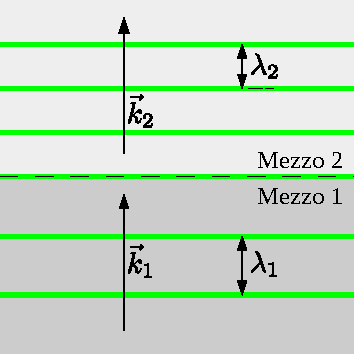
\includegraphics{img/incidenza_normale.pdf}
		\caption{I piani equifase, evidenziati in verde, riducono la distanza tra loro, ovvero la lunghezza d'onda $\lambda_2 < \lambda_1$ nel caso $n_2 > n_1$.}
		\label{fig:incidenza_normale_isolanti}
	\end{figure}

	Nel caso invece di incidenza con un angolo $\theta_i$ rispetto alla normale della superficie, il comportamento è più complesso, come si può osservare in \autoref{fig:incidenza_non_normale_isolanti}.

	La continuità dei piani equifase ci permette ancora di valutare il comportamento dell'onda anche senza risolvere le equazioni di Maxwell.

	Considerando il segmento $l$ evidenziato in figura, la sua lunghezza può essere calcolata in due modi diversi, grazie alle proprietà dei triangoli rettangoli.

	\begin{esp} \label{eq:legge_di_schnell}
		l = \frac{\lambda_1}{\sin(\theta_i)} = \frac{\lambda_2}{\sin(\theta_t)}
	\end{esp}

	\begin{figure}[ht]
		\centering
		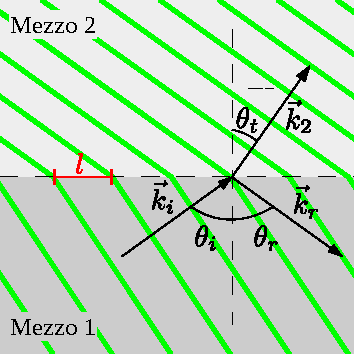
\includegraphics{img/incidenza_non_normale.pdf}
		\caption{La continuità dei campi tangenti impone che i piano equifase conservino la stessa distanza $l$ tra loro \emph{sulla superficie di separazione}.}
		\label{fig:incidenza_non_normale_isolanti}
	\end{figure}

	Nel caso i due elementi abbiamo lo stesso indice di rifrazione $n_i$, l'onda procede senza variazioni: per $\lambda_1 = \lambda_2$ vale infatti che $\theta_1 = \theta_2$.
	Possiamo osservare che questo è ciò che accade per l'onda riflessa, per la quale $\theta_i = \theta_r$, appunto perché l'onda non cambia materiale di propagazione.

\subsection{Coefficienti di riflessione e trasmissione}
	Nella sezione precedente abbiamo osservato come individuare le direzioni dell'onda riflessa e di quella trasmessa: ci focalizzaremo quindi su come la discontinuità influenzi il modulo del campo elettromagnetico.

	Per semplicità di calcolo e notazione ci metteremo nel caso di incidenza normale, ma analogamente segue per il caso generale.

	\begin{figure}[ht]
		\centering
		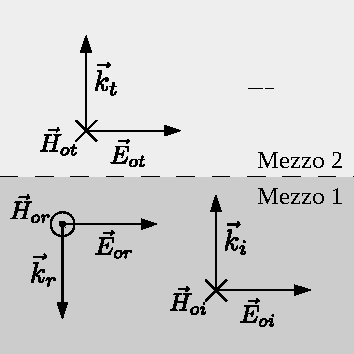
\includegraphics{img/campi_incidenza_normale.pdf}
		\caption{Nella riflessione il campo $\E$ mantiene la sua direzione, mentre $\H$ la inverte. Questo è dovuto ad un asimmetria delle equazioni di Maxwell legata al teorema delle immagini.}
		\label{fig:campi_incidenza_normale_isolanti}
	\end{figure}

	Nella superficie di discontinuità i campi sono tutti paralleli, quindi le somme vettoriali si riducono a somme scalari.
	\begin{esp}
		\begin{cases}
			E_{_0 i} + E_{_0 r} = E_{_0 t} \\
			H_{_0 i} - H_{_0 r} = H_{_0 t}
		\end{cases} \implies
		\frac{E_{_0 i}}{\eta_1} - \frac{E_{_0 r}}{\eta_1} = \frac{E_{_0 t}}{\eta_2} = \frac{E_{_0 i} + E_{_0 r}}{\eta_2}
	\end{esp}
	dove sono state impiegate le formule che legano $|\E|$ e $|\H|$ nel caso dell'onda piana.

	Riorganizzando i termini dell'equazione, si ottiene il \emph{coefficiente di riflessione} $\rho$.
	\begin{esp} \label{eq:coefficiente_riflessione}
		& \rho \stackrel{.}{=} \frac{E_{_0 r}}{E_{_0 i}}
			= \frac{\eta_2 - \eta_1}{\eta_2 + \eta_1}
			\stackrel{(*)}{=} \frac{ \frac{\eta_{_{0}}}{n_2} - \frac{\eta_{_{0}}}{n_1}}{\frac{\eta_{_{0}}}{n_2} + \frac{\eta_{_{0}}}{n_1}}
			= \frac{n_2 - n_1}{n_2 + n_1}
	\end{esp}
	dove (*) vale solamente per i dielettrici, materiali per cui $\eta_i = \frac{\eta_{_{0}}}{n_i}$.

	Il \emph{coefficiente di trasmissione} $\tau$ si può ricavare in modo analogo.
	\begin{esp}
		& \tau \stackrel{.}{=} \frac{E_{_0 t}}{E_{_0 i}}
				= \frac{E_{_0 r} + E_{_0 i}}{E_{_0 i}}
				= \frac{E_{_0 r}}{E_{_0 i}} + 1
				= \rho + 1 \\
	\end{esp}

\subsection{Potenza trasmessa e riflessa}
	A partire dai valori del campo elettrico trasmessi e riflessi è possibile calcolare come si distribuisca la potenza dell'onda nei due materiali.

	\begin{esp}
		I_t
		& = |\Re[\vec{P}]|
			= \frac{|E_{_0 t}|^2}{2 \eta_2}
			= \frac{|E_{_0 i} (1 + \rho)|^2}{2 \eta_2} \\
		& = \frac{|E_{_0 i}|^2}{2 \eta_1} \frac{\eta_1}{\eta_2} |1 + \rho|^2
			= I_i \frac{\eta_1}{\eta_2} |1 + \rho|^2 \\
		& = I_i \frac{4 \eta_1 \eta_2}{|\eta_1 + \eta_2|^2}
			= I_i (1 - |\rho|^2) = I_i - I_i |\rho|^2 = I_i - I_r
	\end{esp}

	È possibile osservare come tutto il comportamento in potenza sia dovuto al solo parametro $\rho$, che definisce sia l'intensità dell'onda trasmessa che quella riflessa.

\subsection{Interferenza in riflessione}
	Come è possibile notare in \autoref{fig:campi_incidenza_normale_isolanti}, nel secondo mezzo c'è un'unica onda che si propaga, mentre nel primo ce ne sono due.
	Questo dà vita a fenomeni di interferenza tra l'onda progressiva incidente e l'onda regressiva riflessa generata dalla discontinuità di mezzo.

	\begin{figure}[ht]
		\centering
		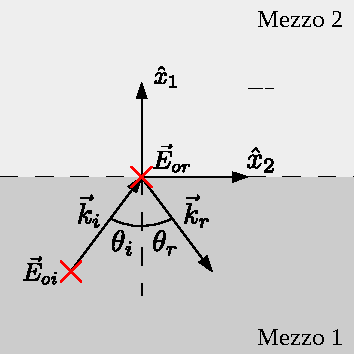
\includegraphics{img/campi_incidenza_non_normale.pdf}
		 \caption{Per l'onda considerata, i campi elettrici sono evidenziati per renderli più visibili e risultano paralleli all'asse $\hat{x}_3$ entrante nel foglio.}
		\label{fig:campi_incidenza_non_normale_isolanti}
	\end{figure}

	Nel caso generico di incidenza, abbiamo che
	\begin{esp}
		\begin{dcases}
			\k_i = (+ \beta_1 \cos(\theta_1), + \beta_1 \sin(\theta_1), 0) \\
			\k_r = (- \beta_1 \cos(\theta_1), + \beta_1 \sin(\theta_1), 0)
		\end{dcases}
	\end{esp}
	dove i vettori sono scomposti nelle loro componenti secondo il sistema di coordinate in \autoref{fig:campi_incidenza_non_normale_isolanti}.

	Il campo nel mezzo 1 si può perciò scrivere come
	\begin{esp}
		\E_1(\r)
		& = \E_{_0 i} ~ e^{-\jmath \k_i \cdot \r} + \E_{_0 r} ~ e^{-j \k_r \cdot \r} \\
		& = E_{_0 i} ~ \hat{x}_3
			~ e^{-\jmath \beta_1 [ \cos(\theta_i) \, x_1 + \sin(\theta_i) \, x_2] }
			+ E_{_0 r} ~ \hat{x}_3
			~ e^{-\jmath \beta_1 [-\cos(\theta_i) \, x_1 + \sin(\theta_i) \, x_2] } \\
		& = E_{_0 i} ~ \hat{x}_3
			~ e^{-\jmath \beta_1 [ \cos(\theta_i) x_1 + \sin(\theta_i) x_2] }
			+ E_{_0 i} (1 + \rho)
			~ \hat{x}_3 ~ e^{-\jmath \beta_1 [-\cos(\theta_i) x_1 + \sin(\theta_i) x_2]} \\
		& = E_{_0 i} (1 + \rho ~ e^{\jmath 2 \beta_1 \cos(\theta_i) x_1} )
			~ e^{-\jmath \beta_1 [\cos(\theta_i) x_1 + \sin(\theta_i) x_2]} \\
	\end{esp}

	Il modulo quadro del campo elettrico oscilla in funzione della posizione $x_1$, alternando piani di interferenza distruttiva (campo nullo) a piani di interferenza costruttiva (campo massimo).

	In particolare, nel caso di incidenza normale si ha che
	\begin{esp}
		|\E_1(\r)|^2
			& = |E_{_0 i}|^2 |1 + \rho ~ e^{\jmath 2 \beta_1 x_1}|^2 \\
			& = |E_{_0 i}|^2
				(1 + \rho ~ e^{\jmath 2 \beta_1 x_1})
				(1 + \rho^* ~ e^{-\jmath 2 \beta_1 x_1}) \\
			& = |E_{_0 i}|^2 (1 + \rho^2 + 2 \rho \cos(2 \beta_1 x_1)) \\
	\end{esp}

	Questi piani individuano lungo $\hat{x}_3$ settori in cui l'impedenza vista dall'onda elettromagnetica varia. Essa, nel caso dell'onda piana, può essere calcolata sfruttando la legge di Ohm.

	\begin{esp}
		Z(x_3)
		& = \frac{E(x_3)}{H(x_3)}
			= \frac
				{E_{_0 i} (1 - e^{\jmath 2 \beta_1 x_3}) ~ e^{- \jmath \beta_1 x_3}}
				{-\frac{E_{_0 i}}{\eta_1} (1 + e^{\jmath 2 \beta_1 x_3}) ~ e^{- \jmath \beta_1 x_3} } \\
		& = \eta_1 ~ \frac
			{e^{\jmath \beta_1 x_3} - e^{\jmath \beta_1 x_3}}
			{e^{\jmath \beta_1 x_3} + e^{\jmath \beta_1 x_3}} \\
		& = \frac{\eta_1}{\jmath} ~ \frac{\sin(\beta_1 x_3)}{\cos(\beta_1 x_3)}
			= -\jmath \, \eta_1 \tan(\beta_1 x_3)
	\end{esp}

	Periodicamente ogni $\lambda_1 / 2$ l'impedenza d'onda oscilla da 0 a $+\infty$:

	\begin{esp}
		\forall m \in \mathbb{N}, ~
		\begin{dcases}
			Z \left( x_3 = -\frac{\lambda_1}{4} - m \frac{\lambda_1}{2} \right) = +\infty
				& \text{circuito aperto} \\
			Z \left( x_3 = - m \frac{\lambda_1}{2} \right) = 0
				& \text{perfetto conduttore} \\
		\end{dcases}
	\end{esp}

\subsection{Riflessione su un buon conduttore}
	Richiamando i risultati ottenuti nella sezione \ref{sec:onda_piana_conduttore}, se il mezzo di trasmissione (mezzo 2) è un buon coduttore, vale che

	\begin{esp}
		\begin{cases}
			|\a| \simeq |\k| = \sqrt{\pi f \mu_{_{0}} \sigma} \\
			\lambda_2 \ll \lambda_1
		\end{cases}
	\end{esp}

	La legge di Schnell, dimostrata in precedenza nell'equazione \eqref{eq:legge_di_schnell}, vale anche in questo caso, ed emerge che la trasmissione è sostanzialmente normale anche per angoli di incidenza diversi da $0^\circ$.

	\begin{esp}
		\sin(\theta_t)
			= \frac{\lambda_2}{\lambda_1} \sin(\theta_t)
			= \begin{cases}
				0 & \theta_i = 0 \\
				\sim 0 & \theta_i \simeq 0
			\end{cases}
			\text{\quad perché } \lambda_2 \ll \lambda_1
	\end{esp}

	Inoltre si può dimostrare come un buon conduttore si comporti come uno specchio per l'onda elettromagnetica, infatti, richiamando l'equazione \eqref{eq:coefficiente_riflessione}, si ha che

	\begin{esp}
		\rho
			= \frac{Z_w - \eta_1}{Z_w + \eta_1}
			= \frac{R_s (1 + \jmath) - \eta_1}{R_s (1 + \jmath) + \eta_1}
			\simeq -1
	\end{esp}
	dove l'ultimo passaggio è giustificato dal fatto che, per i buoni conduttori, la resistenza di parete $R_s$ è molto più piccola dell'impedenza del mezzo isolante $\eta_1$.

	Per esempio, nel passaggio dell'onda dall'aria al rame, si può calcolare che
	\begin{esp}
		\begin{cases}
			R_s = \sqrt{\frac{\pi f \mu_{_{0}}}{\sigma}} \simeq 60m\Omega \\
			\eta_1 = \frac{\eta_{_{0}}}{n_1} \simeq 377\Omega \gg R_s
		\end{cases}
	\end{esp}

	Con valore di $\rho$ come questo, si ha che $I_t = I_i (1 - |\rho|^2) \simeq 0$: il nostro materiale è un buono specchio e diventa uno specchio perfetto per $\sigma \to +\infty$.

%%% Local Variables:
%%% mode: latex
%%% TeX-master: "antenne"
%%% End:

\section{Propagazione guidata}%
Le equazioni delle onde piane uniformi trovate sinora si possono quindi applicare anche per la propagazione di onde elettromagnetiche in conduttori, per esempio
\begin{itemize}%
  \item \textbf{linee bifilari} come il doppino telefonico
  \item \textbf{linee coassiali}, per esempio  cavo che collega l'antenna al televisore
  \item \textbf{le guide rettangolari}, usate principalmente per applicazioni in cui è necessario trasportare molta potenza (radar o trasmissioni satellitari)
  \item \textbf{le linee a microstriscia} utilizzate per trasportare segnali in circuiti stampati
\end{itemize}
Accenniamo ora come si propaga l'onda in alcune di queste guide, poiché il segnale prima di essere emesso dall'antenna dovrà essere trasportato in una qualche maniera.
\paragraph{Campi nella guida}

I campi elettromagnetici che si propagano in guide d'onda il vettore di propagazione  e l'impedenza d'onda sono:
\begin{esp}
  |\k| &=\beta= \omega \sqrt{\mu \epsilon} \\
  \eta &= \frac{E_o}{H_o} = \sqrt{\frac{\mu}{\epsilon}}
\end{esp}

\paragraph{Linea bifilare}
Le linee di forza del campo elettrico nella linea bifilare sono simili a quelle di un condensatre, ossia $\forall$ punto $\E\perp\H\perp\k$. In figura \#TODO\# sono rappresentate le linee di campo.

\paragraph{Linea coassiale}
In questo caso le linee di campo elettrico sono ortogonali alla circonferenza, mentre quelle di campo magnetico sono concentriche all'asse della linea, come visibile in fig \#TODO\#

\paragraph{Impedenza caratteristica}
Cerchiamo ora di valutare l'impedenza caratteristica della linea e, in particolare, come sfruttarla per ridurre al minimo le perdite.

La tensione e la corrente nella linea coassiale si possono scrivere come
\begin{esp}
  V&= \int_{r_{int}}^{r_{ext}} \E \cdot d\vec{l} \\
  I&= \oint \H \cdot d\vec{l} \\
  &\implies Z_c = \frac{V_o}{I_o} \text{ impedenza caratteristica della linea}
\end{esp}
Definendo inoltre
\begin{itemize}
  \item $l$ l'induttanza per unità di lunghezza $\frac{H}{m}$
  \item $c$ la capacità per unità di lunghezza $\frac{F}{m}$
\end{itemize}
si ottiene che l'impedenza caratteristica risulta
\begin{equation}
  Z_c = \sqrt{\frac{l}{c}} = \underbrace{F_{forma}}_{\text{fattore di forma}} \cdot \sqrt{\frac{\mu}{\epsilon}}
\end{equation}

Possiamo quindi riscrivere le equazioni per la tensione e la corrente nel cavo coassiale come
\begin{esp}
  V(z) &= V_o \cdot e^{-\jmath \beta \cdot z}\\
  I(z) &= I_o \cdot e^{-\jmath \beta \cdot z}
\end{esp}


\chapter{Antenne}
In questo capitolo analizzeremo le antenne, partendo inizialmente con i potenziali elettromagnetici e cercando di modificare le equazioni di Maxwell affinché siano più comode da studiare nei nostri casi. Vedremo quindi l'equazione di Helmoltz e la scelta di Lorentz. Inizieremo quindi a studiare le antenne partendo dal caso del dipolo elementare, ideale e non realizzabile nella realtà, ma utile per fare le prime approssimazioni. Estenderemo quindi il dipolo elementare al dipolo corto per studiare poi le antenne lineari, le schiere e le patch.

Riprendiamo le equazioni di Maxwell scritte con i vettori di Steinmets:
\begin{equation}\begin{cases}
  \rot\E = -\jmath \omega \mu\H(\r) \textcolor[rgb]{0.8,0,0}{+ \M} \\
  \rot\H = \jmath  \omega \epsilon \E + \J\\
  \diverg\H=0\\
  \diverg \E = \frac{\rho}{\epsilon}
\end{cases}\end{equation}
Ora aggiungiamo un termine $\M$ fittizio, affinché le equazioni risultino simmetriche e si possano scrivere, in seguito, le equazioni per le sorgenti equivalenti. ($\M$ non può esistere, in quanto non esiste il monopolo magnetico)

\subsubsection{Potenziali elettromagnetici}
$\forall \A , \diverg(\rot \A) = 0$ per quanto trovato nel paragrafo dell'identità notevole (\ref{sec:id-not}). Definiamo quindi $\A$  \textbf{potenziale vettore magnetico} il campo per cui $\H = \frac{1}{\mu} \cdot \rot \A$.
\paragraph{Teorema di Helmoltz}
Un campo vettoriale $\A$ è univocamente definito se sono fissati $\rot \A$ e $\diverg \A$
----------------

Dobbiamo dunque definire in maniera intelligente $\diverg \A$:
\begin{esp} \label{eq:AE}
  \rot\E &= - \jmath \omega \cdot \mu \frac{1}{\mu} \rot \A \quad \Leftrightarrow \quad \rot\left(\rot \E + \jmath \omega \A\right)=0 \\
  \forall \Phi& \text {, scalare, } \rot(\diverg\Phi)=0\\
  \E +& \jmath \omega \A = -\nabla\Phi \quad \implies \E = -\jmath \omega \A - \nabla \Phi  \\
  \implies &[\Phi] = V
\end{esp}
Definiamo quindi $\Phi$ potenziale scalare elettrico associato ad $\A$. Analizziamo ora la seconda equazione di Maxwell
\begin{esp}
  \rot \H &= \jmath \omega \epsilon_c \cdot \E + \J \\
  \mu \cdot \rot\left(\frac{1}{\mu} \rot \A\right) &= \jmath \omega \mu \epsilon_c \cdot \left(-\jmath \omega \A - \nabla \Phi \right) + \J \mu  \\
  -\nabla^2\A + \diverg(\nabla \A) = \omega^2 \mu \epsilon_c \A - \jmath \omega \mu \epsilon_c \nabla \Phi + \mu \J \\
  \underbrace{\nabla^2 \A + \omega^2 \mu \epsilon_c \A}_{\parbox[c]{2cm}{\text{Struttura dell'eq. di Helmoltz}}} &= -\mu\J + \diverg(\nabla\A) + \jmath \omega \mu \epsilon_c \nabla \Phi \\
  &=\underbrace{-\mu\J}_{\parbox[c]{2cm}{\text{termine noto: presenza sorgenti}}} + \diverg\left(\underbrace{\nabla \A + \jmath \omega \mu \epsilon_c \Phi}_{\parbox[c]{2cm}{\text{complicazione? scelgo il valore di $\A$}}}\right)\\
\end{esp}
\paragraph{Scelta di Lorentz}
Poiché abbiamo ancora un grado di libertà per definire $\A$, possiamo scegliere
\begin{equation}
  \diverg \A = -\jmath \omega \mu \epsilon_c \Phi
\end{equation}
Otteniamo quindi l'\textbf{equazione di Helmoltz non omogenea}:
\begin{equation}
  \nabla^2\A + \omega^2 \mu\epsilon_c\A =-\mu \J
\end{equation}
Dobbiamo quindi determinare il valore di $\Phi$, cosa che faremo sfruttando la terza legge di Maxwell
\begin{esp*}
  \diverg\E &= \frac{\rho}{\epsilon} \quad \implies\quad \diverg\left(-\jmath \omega \A - \nabla \Phi  \right)= \frac{\rho}{\epsilon}\\
  \implies & \jmath \omega \A + \nabla \Phi= -\frac{\rho}{\epsilon}  \\
  &\jmath\omega\left(-\jmath \omega\mu\epsilon_c\Phi\right) + \nabla^2\Phi = - \frac{\rho}{\epsilon}\\
  &\text{Otteniamo quindi l'equazione scalare di Helmoltz non omogenea}\\
  &\omega^2\mu\epsilon_c\Phi + \nabla^2 \Phi = -\frac{\rho}{\epsilon}
\end{esp*}
\begin{esp}\label{eq:helmolts-lorentz}
  \nabla^2\A + \omega^2\mu\epsilon_c\A &= -\mu\J \\
  \nabla^2\Phi + \omega^2\mu\epsilon_c\Phi &= -\frac{\rho}{\epsilon}
\end{esp}
Poiché le equazioni di Helmoltz trovate sono lineari, utilizzeremo spesso il principio di sovrapposizione degli effetti

\section{Dipolo elementare}
Partiamo analizzando il dipolo elementare, indicando la rappresentazione di un punto P attraverso il vettore posizione $\r$
\begin{esp}
  \r &= (x,y,z) = (|\r|,\theta,\phi) = (r,\theta,\phi) \\
  \J &= I \cdot \delta(x)\delta(y)\cdot f(z)\cdot \hat{z}
\end{esp}
Dobbiamo quindi risolvere l'equazione di Helmoltz non omogenea:
\begin{esp*}
  \nabla^2 \A + \omega^2 \mu\epsilon_c \A &= -\mu \J \quad \text{con } \A = (A_x,A_y,A_z)\\
  \begin{cases}
    \nabla^2 \A_{x,y} + \omega^2 \mu\epsilon_c\A_{x,y} =0 \\
    \nabla^2 \A_{z} + \omega^2 \mu\epsilon_c\A_{z} =-\mu\J_z
  \end{cases} \\
  \implies & A_x=A_y=0 \parbox[c]{5cm}{\text{ è una soluzione possibile e più semplice}}\\
  \forall \r &= 0 \implies \nabla^2 \A_{z} + \omega^2 \mu\epsilon_c\A_{z} =0
\end{esp*}
Supponiamo ora che $\sigma=0 \implies \epsilon_c = \epsilon \in \R$
\begin{equation*}
  \nabla^2 \A_{z} + \omega^2 \mu\epsilon\A_{z} =0
\end{equation*}

Le soluzioni dovranno avere simmetria sferica
\begin{esp*}
  &A_z(r,\theta,\phi) =A_z(r) = \frac{f(r)}{r} \\
  &\implies \nabla^2 A_z = \frac{1}{r^2} \deriv{}{r}\left(r^2 \deriv{A_z(r)}{r}\right) \\
  &\implies  \frac{1}{r^2} \deriv{}{r}\left(r^2 \deriv{\frac{f(r)}{r}}{r}\right) + \omega^2 \mu\epsilon\frac{f(r)}{r}\\
  & \frac{1}{r} \deriv{}{r}\left(r^2 \deriv{\frac{f'(r)\cdot r - f}{r^2}}{r}\right) + \omega^2 \mu\epsilon\frac{f(r)}{r}\\
  &\frac{1}{r} \cdot \left(f\prime\prime(r)\cdot r + f\prime(r)\cdot 1 - f\prime(r) \right) + \omega^2\mu\epsilon f(r) = 0\\
\end{esp*}
dove $f\prime(r) = \deriv{f(r)}{r}$ e $f\prime\prime =\deriv[2]{f(r)}{r}$
Concludiamo quindi che
\begin{equation*}
  f\prime\prime(r) + \omega^2\mu\epsilon f(r) = 0
\end{equation*}
Integrando otteniamo
\begin{equation}
  f(r) = c \cdot e^{-\jmath \beta r} + d \cdot e^{\jmath \beta r}
\end{equation}
con $c,d \in \C$ costanti di integrazione, $\beta = \omega\sqrt{\mu\epsilon}$.

$A_z(r)$ risulta quindi essere
\begin{equation}
  A_z(r) = \frac{c}{r}\cdot e^{-\jmath \beta r} +\frac{d}{r}\cdot e^{\jmath \beta r}
\end{equation}
che non è più un'onda piana.

Nel dominio temporale, ora troviamo che:
\begin{equation}
  a_z(r,t) = \Re \left[A_z(r)\cdot e^{\jmath \omega t}\right] \propto cos(\omega t \pm \beta r)
\end{equation}
che rende evidente come non ci sia dipendenza rispetto $\theta$ e $\phi$. Questo implica che l'onda si propaga radialmente. Il $\pm$ indica la presenza di un'onda progressiva e, eventualmente, una regressiva, la quale si annulla se non vi sono ostacoli.

Definiamo ora la velocità di fase: $v_f = \frac{\omega}{\beta}$
Analizzando $A_z$ otteniamo che
\begin{itemize}
  \item $|A_z| = \left|\frac{c}{r}\right|$ la superficie equiampiezza è una sfera di raggio r
  \item $\measuredangle A_z = \beta r$ la superficie equifase è una sfera di raggio r
\end{itemize}
ossia l'onda è di tipo sferico.

integrando nel volume della sfera otteniamo
\begin{esp*}
  \int_V \nabla^2 A_z \cdot dV + \omega^2 \mu \epsilon \int_V A_z \cdot dV &= -\mu \int_V J_z \cdot dV \\
  \int_V \diverg(\nabla A_z) \cdot dV + \omega^2 \mu \epsilon \int_V A_z \cdot dV &= -\mu \int_V I \cdot \delta(x)\delta(y)\cdot F(z) \cdot dV \\
  \text{ con } F(z) &=
  \begin{cases}
    1 & |z| \le \frac{\Delta z}{2} \\ 0 &\text{altrove}
  \end{cases}
\end{esp*}
Attraverso il teorema della divergenza possiamo continuare
\begin{esp*}
  \int_{S_V} \nabla A_z \cdot \r \cdot dS + \omega^2 \mu \epsilon \int_V A_z \cdot dV &= -\mu \int_V I \cdot \delta(x)\delta(y)\cdot F(z) \cdot dV \\
  \nabla A_z = \hr \cdot \deriv{A_z}{r} &= \hr \cdot c \left(\frac{-\jmath \beta \ejbr -\ejbr }{r^2}\right) \\
  c \cdot \int_{S_V} \left(-\jmath\beta\frac{\ejbr}{r} -\frac{\ejbr}{r} \right) \hr \cdot \hr dS + \int_V \oqme A_z dV &= -\mu \int_V I \cdot \delta(x)\delta(y)\cdot F(z) \cdot dV \\
  \A_z(r) = \frac{\mu\cdot I \cdot \Delta z}{4\pi}\cdot \frac{\ejbr}{r} \cdot \hz
\end{esp*}
Dove $c=\frac{\mu\cdot I \cdot \Delta z}{4\pi}$, calcolato attraverso il teorema dei residui.

Otteniamo quindi le equazioni per il csmpo elettrico e magnetico
\begin{esp}\label{eq:campoDE}
  \H &= \frac{1}{\mu}  \cdot \rot \A \stackrel{=}{conti} \frac{I \cdot \Delta z}{4\pi} \cdot \left(\frac{\jmath \beta}{r} + \frac{1}{r^2}\right)\cdot\ejbr \cdot sin(\theta)\hphi\\
  \E &= -\jmath\omega\A - \nabla \left(\frac{\diverg\A}{-\jmath\omega\mu\epsilon}\right) \stackrel{=}{conti}\\
  &= \eta \frac{I \cdot \Delta z}{4\pi} \cdot\left(\frac{\jmath \beta}{r} + \frac{1}{r^2} + \frac{1}{\jmath\beta r^3}\right)\cdot\ejbrp \cdot sin(\theta)\hth +
  \eta \frac{I \cdot \Delta z}{2\pi} \cdot\left( \frac{1}{r^2} + \frac{1}{\jmath\beta r^3}\right)\cdot\ejbr \cdot cos(\theta)\hr
\end{esp}

L'andamento della soluzione del campo elettrico permette di individuare la regione di campo lontano, in particolare con le approssimazioni per r sufficientemente grande, si ottiene:
\begin{esp*}
  \frac{\jmath\beta}{r} &= \frac{\jmath 2\pi}{\lambda \cdot r} \quad \lambda r \gg  \lambda \implies \text{regione campo lontano}\\
  \frac{1}{\jmath\beta r^3} &= \frac{\lambda}{\jmath 2 \pi r^3} \to 0 \\
  \H &\approx \frac{I \cdot \Delta z}{4\pi} \cdot \frac{\jmath\beta}{r} \cdot \ejbr sin(\theta)\hphi\\
  \E &\approx \eta \cdot \frac{I \cdot \Delta z}{4\pi} \cdot \jmath\beta\cdot \frac{\ejbr{r}}{r} sin(\theta) \cdot \hth
\end{esp*}

Possiamo quindi scrivere le condizioni di campo lontato:
\begin{equation}\begin{cases}
  E_\theta \approx \jmath\beta\eta\cdot\frac{I \cdot \Delta z}{4\pi} \cdot \frac{\ejbr}{r} \cdot sin(\theta) = \jmath \eta\cdot\frac{I \cdot \Delta z}{2\lambda} \cdot \frac{\ejbr}{r} \cdot sin(\theta) \\
  E_\theta \approx \jmath\beta\cdot\frac{I \cdot \Delta z}{4\pi} \cdot \frac{\ejbr}{r} \cdot sin(\theta) = \jmath \cdot\frac{I \cdot \Delta z}{2\lambda} \cdot \frac{\ejbr}{r} \cdot sin(\theta) \\
\end{cases}\end{equation}

Possiamo quindi trovare una relazione tra l'impedenza d'onda e il campo EM, attraverso
\begin{equation}
  \frac{E_\theta}{H_\Phi} = \eta \in \R
\end{equation}
L'onda è quindi localmente piana.

Il vettore di Poynting risulta quindi
\begin{esp*}
  \S = \frac{\E \times\H^*}{2} &= \frac{E_\theta \cdot \hth \times H_\Phi \cdot \hphi}{2} = \frac{E_\theta\cdot H_\Phi}{2}\cdot \hth \times \hphi \\
  &= \frac{E_\theta\cdot H_\Phi}{2} \cdot \hr = \frac{\eta|I|^2 \Delta z^2}{8\lambda^2\r^2} \sin^2(\theta)\cdot \hr \\
  &=\frac{\eta |I|^2}{8} \cdot \left(\frac{\Delta z}{\lambda}\right)^2 \cdot \frac{sin^2(\theta)}{r^2} \cdot \hr = \Re[\P]
\end{esp*}
dove $\Re[\P]$ è il flusso di potenza attiva.

\paragraph{Efficienza di radiazione del dipolo elementare}

Dimostriamo ora che il dipolo elementare non è un'antenna efficiente e per farlo analizzeremo la potenza irradiata($P$) utilizzando il vettore di Poynting($\P$). Definiamo $S(r)$ la superficie della sfera di raggio r e $I(r,\theta,\Phi)$ l'intensità di radiazione del campo in un punto della sfera di raggio $r$ e coordinate sferiche $\theta , \Phi$).
\begin{esp*}
  P &= \int_{S(r)} \Re[\P] \cdot \hr \cdot dS = \int_{S(r)} I(r,\theta,\Phi)\cdot \underbrace{\hr \cdot \hr}_{=1} dS \\
  &= \int_0^{2\pi}\int_0^\pi I(r,\theta,\Phi)\cdot r^2 \cdot sin(\theta) \cdot d\theta \cdot d\Phi \\
  &= \int_0^{2\pi}\int_0^\pi \frac{\eta |I|^2}{8} \cdot \left(\frac{\Delta z}{\lambda}\right)^2 \cdot \frac{sin^2(\theta)}{r^2} \cdot r^2 sin(\theta) d\theta \cdot d\Phi \\
  &=\frac{\eta |I|^2}{8} \cdot \left(\frac{\Delta z}{\lambda}\right)^2 \cdot 2\pi \cdot  \underbrace{\int_0^\pi sin^3(\theta)}_{=\frac{4}{3}} = \frac{\pi}{3} \eta |I|^2 \left(\frac{\Delta z}{\lambda}\right)^2
\end{esp*}

Analizziamo ora il vettore di Poyting per vedere come si comporta il campo EM in un caso generico, ossia in assenza di approssimazioni di campo lontano.
\begin{esp}
  \P &= \frac{\E \times \H^*}{2} = \frac{1}{2} \cdot (E_\theta \hth + E_r \hr) \times H_\Phi^* \hphi \\
  &=\frac{1}{2} \cdot \eta \frac{|I|^2 \cdot (\Delta z)^2}{(4\pi)^2} \cdot\left(\frac{\jmath \beta}{r} + \frac{1}{r^2} + \frac{1}{\jmath\beta r^3}\right) \cdot sin^2(\theta) \left(\frac{-\jmath \beta}{r} + \frac{1}{r^2}\right)\hr \\
  &+\frac{1}{2} \cdot \eta \frac{|I|^2 \cdot (\Delta z)^2}{2\pi\cdot 4\pi} \cdot\left( \frac{1}{r^2} + \frac{1}{\jmath\beta r^3}\right) \cdot cos(\theta)\cdot sin(\theta)\left(\frac{-\jmath \beta}{r} + \frac{1}{r^2}\right)\cdot(-\hth)\\
  &= \eta \frac{|I|^2 \cdot (\Delta z)^2}{32\pi^2} sin^2(\theta) \cdot \left(\frac{\beta^2}{r^2}+\frac{\jmath\beta}{r^3}-\frac{\jmath\beta}{r^3} +\frac{1}{r^4}-\frac{1}{r^4} + \frac{1}{\jmath\beta r^5}\right) \hr \\
  &-\eta \frac{|I|^2 \cdot (\Delta z)^2}{16\pi^2} sin(\theta)\cos(\theta) \cdot \left(-\frac{\jmath\beta}{r^3} +\frac{1}{r^4}-\frac{1}{r^4} + \frac{1}{\jmath\beta r^5}\right) \hth \\
\end{esp}
Facendo le dovute semplificazioni e scrivendo, dove necessario $\beta = \frac{2\pi}{\lambda}$ otteniamo:
\begin{esp}
  P=\eta \frac{|I|^2 \cdot (\Delta z)^2}{32\pi^2} sin^2(\theta) \cdot \frac{4\pi^2}{\lambda^2} \cdot \left(1+ \underbrace{\frac{1}{\jmath\beta^3 r^3}}_{\frac{1}{\jmath}\left(\frac{\lambda}{2\pi r}\right)^3}\right) \hr
  +\eta \frac{\jmath\beta |I|^2 \cdot (\Delta z)^2}{16\pi^2\cdot r^3} sin(\theta)\cos(\theta) \cdot \left(1 - \frac{1}{(\jmath\beta)^2 r^2}\right) \hth \\
\end{esp}
Osservando ora la parte immaginaria otteniamo:
\begin{equation}
  \Im[\P] = -\jmath\frac{\eta}{\beta} |I|^2 \cdot \left(\frac{\Delta z}{4\pi}\right)^2 \cdot \frac{1}{r^5}\left(sin^2(\theta)\hr - sin(2\theta)\hth\right)
\end{equation}
Il comportamento della parte immaginaria è mostrato in figura \ref{fig:capIndutt}
\begin{figure}\centering
  % \documentclass{standalone}
% \usepackage[usenames,dvipsnames,table,tikz]{xcolor} % use colors on table and more
% \usepackage{tikz}
%
% \usepackage{pgfplots}
% \begin{document}
\begin{tikzpicture}\begin{axis}[axis lines=middle,samples=200
        ,xlabel=$\theta$
        ,ymax=1.2
        ,ymin=-1.2
        ,xmin = -0.05
        ,xmax = 3.5
        ,every axis x label/.style={
          at={(ticklabel* cs:1.05)},
            anchor=west,
          },
        every axis y label/.style={
          at={(ticklabel* cs:1.05)},
            anchor=south,
          },
        ,xtick=data
        ,xtick={-0.05,1.045,3.141592}
        ,xticklabels={0,A,$\pi$}
        ,ytick=data,
        ,ytick={1,-1}
        ,yticklabels={1,-1}
        ,legend style={at={(axis cs:0.2,-0.5)},anchor=north west}
        ]
      \addplot[red,domain=0:3.141592] {sin(deg(x)};
      \addplot[blue,domain=0:3.141592] {sin(deg(2*x))};
      \addplot[gray,dotted,mark=none] coordinates {(1.045, 0) (1.045, 1)};
      \legend{$sin(\theta$),$sin(2\theta$)}
\end{axis}\end{tikzpicture}
% \end{document}

  \caption{Dall'origine al punto A il comportamento di $\Im[\P]$ è induttivo, tra A e $\pi$ è capacitivo}
  \label{fig:capIndutt}
\end{figure}

\section{Parametri di un'antenna}
Mostreremo ora i parametri attraverso cui un'antenna è caratterizzata, prima elencandoli e poi ricavandoli per il dipolo elementare.
I parametri, dunque, sono
\begin{itemize}
  \item Pattern di radiazione in campo e in potenza
  \item SLL - Side Lobe Level
  \item Direttività
  \item Guadagno in potenza
\end{itemize}

\subsection{Pattern di radiazione}
\paragraph{Pattern di radiazione in campo}
Si definisce Pattern di radiazione in campo il rapporto
\begin{equation} \label{eq:patternCampo}
  F(\theta,\Phi) = \frac{E_\theta(r,\theta,\Phi)}{E_\theta(r,\theta_{max},\Phi_{max})}
\end{equation}
dove
\begin{equation}
  \{\theta_{max} , \Phi_{max}\} = \max_{\theta,\Phi} |E_\theta(r,\theta,\Phi)|
\end{equation}

Nel caso del dipolo elementare, si ha:

\begin{equation}
  F_{DE}(\theta,\Phi) = \frac{\jmath\eta I \frac{\Delta z}{\lambda} \frac{\ejbr}{r} sin(\theta)}{\jmath\eta I \frac{\Delta z}{\lambda} \frac{\ejbr}{r}} = sin(\theta) \, \theta_{max}=\frac{\pi}{2} \implies sin(\theta_{max}) =1
\end{equation}


\paragraph{Pattern di radiazione in potenza}
Definiamo il pattern di radiazione in potenza come
\begin{equation}\label{eq:patternPotenza}
  P(\theta,\Phi) = |F(r,\theta,\Phi)|^2 = \frac{|E_\theta(r,\theta,\Phi)|^2}{|E_\theta(r,\theta_{max},\Phi_{max})|^2} = \frac{|I|}{|I_{max}|} \, 0\le P(\theta,\Phi) \le 1
\end{equation}

Nel caso del dipolo elementare si ha che il pattern di radiazione in potenza è
$|  F_{DE}(\theta,\Phi)|^2 = sin^2(\theta)$

\subsection{Side Lobe Level SLL}
Definiamo il rapporto dei lobi secondari come
\begin{equation}\label{eq:SLL}
  SSL=10 \cdot log_{10}\left|\frac{F(SSL)}{F_{max}}\right|^2 = 20 \cdot log_{10} |F(SSL)|
\end{equation}
tenendo a mente che $F_{max}=1$

\paragraph{Solidi di direttività}
Dal pattern di radiazione in campo e in potenza, possiamo trovare i solidi di direttività in campo lontano. Il solido di direttività è un grafico tridimensionale che in coordinate sferiche permette di valutare la propagazione. Nel caso del dipolo elementare i suoi solidi di direttività in campo e in potenza sono visibili in figura \ref{fig:pattern}.
Poiché la maggior parte delle volte risulta difficoltoso rappresentare un grafico tridimensionale che sia facile e veloce da leggere, si decide di rappresentare un grafico bidimensionale, che verrà chiamato \textbf{diagramma di radiazione}.
Il diagramma di radiazione si costruisce omettendo uno dei due angoli $\theta$ o $\Phi$ e utilizzando
\begin{itemize}
  \item coordinate polari, la rappresentazione più utilizzata perché permette di cogliere immediatamente dove il campo si propaga;
  \item coordinate cartesiane, la rappresentazione che dà più risalto all'intensità del campo in determinati angoli.
\end{itemize}

\subsection{Direttività}
Il concetto di direttività di un'antenna è legato al voler quantificare la porzione di potenza che viene emessa nel lobo (o nei lobi) principali rispetto alla potenza media irradiata dall'antenna.
Iniziamo quindi a determinare come la potenza irradiata:
\begin{equation}
  P= \int_{S(r)} I(r,\theta,\Phi) dS =\int_0^\pi\int_0^{2\pi} I(r,\theta,\Phi)\cdot r^2 \cdot sin(\theta)d\theta\,d\Phi
\end{equation}

Definiamo quindi la potenza per unità di angolo solido la quantità
\begin{equation}
  U(\theta,\Phi)=I(r,\theta,\Phi)\cdot r^2 \quad [U] = W = \frac{W}{sterad}
\end{equation}
definiamo inolte il massimo della potenza per unità di angolo solido come:
\begin{equation}
  U_m = \max_{\theta,\Phi} U(\theta,\Phi) = U(\theta_{max},\Phi_{max})
\end{equation}
Possiamo quindi riscrivere la potenza come
\begin{equation}
  \int_0^\pi \int_0^{2\pi} U(\theta,\Phi) \cdot \underbrace{ sin(\theta) d\theta \, d\Phi}_{\text{ \parbox{2cm}{$d\Omega$ unità infinitesima di angolo solido}}}
\end{equation}
Da quest'ultima equazione possiamo definire la potenza media per unità di angolo solido come
\begin{equation}
  U_{AVG} = \frac{1}{4\pi}\cdot \int U(\theta,\Phi) \cdot d\Omega
\end{equation}
Definiamo quindi la direttivià come il rapporto
\begin{equation}
  D=\frac{U_m}{U_{AVG}}
\end{equation}

Possiamo riscrivere la direttività in due altri modi differenti:
\begin{esp}\label{eq:dirett}
  D&\stackrel{=}{1}\frac{I(r,\theta_{max},\Phi_{max})}{\frac{1}{4\pi}\int I(r,\theta,\Phi) sin(\theta) \cdot d\theta \, d\Phi} \\
  &\stackrel{=}{2}\frac{U_m}{\frac{P}{4\pi}} =\frac{U_m\cdot 4\pi}{P} = \frac{4\pi r^2 I(r,\theta_{max},\Phi_{max})}{P}
\end{esp}
La quantità $4\pi r^2 I(r,\theta_{max},\Phi_{max})$ viene normalmente chiamata \textbf{EIRP}: Effective Isotropic Radiated Power e indica un'antenna che trasmetta isotropicamente con un campo pari a quello nella direzione del massimo.

\paragraph{Direttività del dipolo elementare}

Nel dipolo elementare abbiamo che:
\begin{esp*}
  U(\theta,\Phi) &= \frac{\eta \cdot |I|^2}{8} \cdot \left(\frac{\Delta z}{\lambda}\right)^2 sin(\theta) \\
  U_m &= \frac{\eta \cdot |I|^2}{8} \cdot \left(\frac{\Delta z}{\lambda}\right)^2\\
  P&= \frac{\pi}{3}\eta |I|^2 \left(\frac{\Delta z}{\lambda}\right)^2 \\
  \implies & D_{DE} = \frac{U_m \cdot 4\pi}{P}= \frac{\frac{\eta \cdot |I|^2}{8} \cdot \left(\frac{\Delta z}{\lambda}\right)^2 \cdot 4\pi}{\frac{\pi}{3}\eta |I|^2 \left(\frac{\Delta z}{\lambda}\right)^2} = \frac{3}{2} = 1,5
\end{esp*}
Il risultato ottenuto mostra come il dipolo elementare sia poco direttivo. Spesso però si è soliti riportare la direttività in decibel rispetto a un'antenna isotropa (che quindi ha direttività pari a 1): $D_{DE_{dB}} \approx 1.76 dB$

Ipotizziamo ora un'antenna ideale che emette in un settore della sfera, per esempio supponiamo il pattern di radiazione in campo pari a:
\begin{equation}F=\begin{cases}
  1 & \frac{\pi}{3}\le \theta \le\frac{2}{3}\pi \\ 0 & \text{altrove}
\end{cases}\end{equation}
Possiamo scrivere la potenza media per unità di angolo solido come
\begin{equation}
  U_{AVG} =\frac{1}{4\pi}\int U(\theta,\Phi) d\Omega = \frac{U_m}{4\pi}\int |F|^2 d\Omega
\end{equation}

La direttività quindi risulta
\begin{esp*}
  D=\frac{U_m}{U_{AVG}} = 4\pi\frac{U_m}{U_m}\cdot \frac{1}{\int_0^{2\pi}\int_{\frac{\pi}{3}}^{\frac{2}{3}\pi} sin(\theta)d\theta \, d\Phi} = \frac{4\pi}{2\pi} = 2
\end{esp*}
Abbiamo quindi trovato un altro modo per scrivere $U(\theta,\Phi)$:
\begin{equation}
  U(\theta,\Phi) = |F(\theta,\Phi)|\cdot U_m
\end{equation}

Possiamo definire inoltre l'angolo solido del fascio, o \textit{beam solid angle} la quantità
\begin{equation}
  \Omega_A = \int |F(\theta,\Phi)|^2 d\Omega
\end{equation}
Otteniamo quindi che la direttività si può scrivere come
$$D= \frac{4\pi}{\Omega_A}$$.

\textsc{Remark:} a volte si scrive $D(\theta,\Phi) = D \cdot |F(\theta,\Phi)|^2$ rinormalizzando come visto in \eqref{eq:dirett} (2)
\subsection{Guadagno in potenza}
Non sempre si riesce a conoscere in ogni punto il valore di $I(r,\theta,\Phi)$, per cui si procede analizzando la potenza elettrica emessa rispetto alla direttività dell'antenna. In particolare, osservando anche la figura \ref{fig:antDipolo}, si procede come segue:
\begin{esp}
  P_{IN} &= \Re\left[\frac{V_A \cdot I_A^*}{2}\right] \\
  G= \frac{U_m}{\frac{P_{IN}{4\pi}}}
\end{esp}
Poiché si riesce sempre a calcolare
\begin{esp}
  4\pi U_m  &= G \cdot P_{IN} \leftrightarrow 4\pi U_m = D \cdot P\\
  \implies & G=D \frac{P}{P_IN} \quad D =G \frac{P_{IN}}{P}
\end{esp}
Sapendo che non esiste alcun materiale con resistenza nulla, si ha $P \le P_{IN}$. \\
Definiamo quindi efficienza dell'antenna o efficienza di radiazione la quantità
\begin{equation}\label{eq:efficienzaAnt}
  e_r = \frac{P}{P_IN}
\end{equation}

Possiamo ora riscrivere G come
\begin{esp*}
  G&=\frac{4\pi\U_m}{P_{IN}} \cdot \frac{r^2}{r^2} = \frac{4\pi r^2 I(r,\theta,\Phi)}{P_{IN}} = \frac{EIRP}{P_{IN}} \\
  EIRP &= G \cdot P_{IN} = D \dot P \\
  I(r,\theta,\Phi) &= G \frac{P_in}{4\pi r^2}\\
  \implies &G(\theta,\Phi) = G \cdot |F(\theta,\Phi)|^2
\end{esp*}

\section{Impedenza d'antenna}
Vogliamo ora valutare come adattare l'antenna affinché la maggior parte della potenza venga trasmessa e irradiata, invece che venir riflessa nel cavo.
Definiamo quindi l'impedenza di antenna:
\begin{equation}
  Z_A = \frac{V_A}{I_A} = R_A + \jmath \Chi_A
\end{equation}
dove $R_A$ è la resistenza d'antenna e $\Chi_A$ è la reattanza d'antenna.

Possiamo inoltre scrivere la potenza in ingresso all'antenna come:
\begin{esp*}
  P_{IN} &\stackrel{=}{1} \frac{R_A \cdot |I_A|^2}{2} = \Re\left[\frac{V_a \cdot I_A^*}{2}\right] \\
  &\stackrel{=}{2} \underbrace{P}_{pot. irradiata} + \underbrace{P_o}_{pot. dissipata}\\
  &= P + R_o \cdot \frac{|I_A|^2}{2}
\end{esp*}
definendo $R_o$ resistenza ohmica dell'antenna e $R_r$ la  resistenza di radiazione, tale per cui $P=R_r \cdot \frac{|I_A|^2}{2}$

Possiamo quindi ricavare
\begin{esp*}
  P_{IN} &= (R_o + R_r)\cdot \frac{|I_A|^2}{2}\\
  e_r &= \frac{R_r}{R_r + R_o} = \frac{R_r}{R_A} \le 1
\end{esp*}

Nel caso del dipolo elementare, supponendo una resistenza ohmica trascurabile, otteniamo:
\begin{esp*}
  P&=\frac{\pi}{3} \eta |I_A|^2 \cdot \left(\frac{\Delta z}{\lambda}\right)^2 \quad P_{IN} = P \\
  R_r = \frac{2P}{|I_A|^2} = \frac{2}{3}\pi \eta  left(\frac{\Delta z}{\lambda}\right)^2 = 80\pi^2left(\frac{\Delta z}{\lambda}\right)^2 \Omega
\end{esp*}
poiché il rapporto $left(\frac{\Delta z}{\lambda}\right)$ è molto piccolo, l'antenna risulta poco efficiente.
Osserviamo ora la potenza reattiva emessa dall'antenna, in modo da calcolare $\Chi_A$. Iniziamo riprendendo l'equazione \eqref{eq:bilancio_potenza_EM_steinmetz}:
\begin{esp*}
  \Im\left[- \int_V \E \cdot \J^* ~ dV\right] &= \omega \underbrace{\int_V \omega \left[\mu \frac{|\H|^2}{2} - \epsilon \frac{|\E|^2}{2} \right] dV}
    _{<0} + \Im\left[\int_{S(r)} \P \cdot \hr dS\right] \\
  \Im\left[\frac{V_a \cdot I_A^*}{2}\right] &= -\omega\epsilon
\end{esp*}


\end{document}
